\motto{C'est l'harmonie des diverses parties, leur symétrie, leur heureux balancement; c'est en un mot tout ce qui y met de l'ordre, tout ce qui leur donne de l'unité, ce qui nous permet par conséquent d'y voir clair et d'en comprendre l'ensemble en même temps que les détails.

--- Henri Poincaré\footnote{Henri Poincaré (1854--1912) was a French mathematician, physicist, and philosopher of science. He is considered one of the greatest mathematicians of all time and a pioneer of several modern mathematical fields. He also played a key role in the development of special relativity, and was one of the first to understand the deep connection between mathematics and physics.}, \emph{L'avenir des mathématiques}}
\chapter{Toric pluripotential theory on big line bundles}
\label{chap:toric_big}

This chapter extends the toric pluripotential theory of \cref{chap:toric_ample} from ample toric line bundles to big toric line bundles. Let $L=\mathcal O_X(D)$ be a big toric line bundle on a smooth projective toric variety $X$, and let $P_D\subseteq M_{\mathbb R}$ be the polytope associated with the toric divisor $D$. In the ample case, $P_D$ is a smooth lattice polytope and its faces correspond directly to toric strata. This direct correspondence breaks down. This is the main new feature of the chapter.

The first goal is to recover a usable toric-convex dictionary in this more flexible setting. We begin by recalling the big toric setup, the Cartier data of $D$, and the stable base locus. We then compare the Newton body of a toric psh metric with its partial Okounkov body. The main computation, \cref{thm:toricpob}, identifies the partial Okounkov body of a toric singularity with its Newton body, up to the natural affine transformation determined by the chosen toric flag. This result is the bridge between the general Okounkov-body theory of \cref{chap:Okounkov} and the explicit convex geometry of toric metrics.

Once this comparison is established, several pluripotential-theoretic consequences follow. The Newton body computes non-pluripolar mass, describes Lelong numbers along toric divisors, and gives an explicit description of the potential with minimal singularities. In this way the abstract constructions of previous chapters become concrete convex-geometric statements in the toric setting.

The second half of the chapter develops the full toric pluripotential theory in a big class. Toric $\theta$-psh potentials are identified with proper convex functions on $N_{\mathbb R}$ satisfying the appropriate growth condition determined by $P_D$. Under this correspondence, sums, rooftop envelopes, suprema, decreasing limits and $P$-equivalence all have convex interpretations. We also describe toric subgeodesics, geodesics and the toric Ross--Witt Nystr\"om correspondence.

The final sections study restriction and intersection theory in the toric setting. The trace operator along toric strata is computed by slicing Newton bodies, and its volume formula becomes a statement about the Euclidean volume of faces and slices. We also prove a mixed-volume formula for Newton bodies and recover the augmented base locus from the convex data.

Throughout the chapter we use the notation and conventions of \cref{chap:toric_ample}. The partial Okounkov body machinery of \cref{chap:Okounkov} is used repeatedly.


\section{Toric setup}\label{sec:toricsetup2}
Let $T$ be a complex torus of dimension $n$ with character lattice $M$ and cocharacter lattice $N$. Some basic terminology is recalled in \cref{sec:toricsetup}.
Recall that $T_c$ is the compact torus contained in $T(\mathbb{C})$.

Consider a rational polyhedral fan $\Sigma$ in $N_{\mathbb{R}}$ corresponding to an $n$-dimensional smooth projective toric variety $X$.

Let
\[
D=\sum_{\rho\in \Sigma(1)} a_{\rho}D_{\rho}
\]
be a $T$-invariant integral big divisor on $X$. Let $P_D\subseteq M_{\mathbb{R}}$ be the following polytope\footnote{Note that $P_D$ is not necessarily a lattice polytope, see \cite[Example~10.5.4]{CLS11}. In fact, any rational polytope with positive volume can be realized in this manner.}
\begin{equation}\label{eq:bigPrep}
P_D=\left\{ m\in M_{\mathbb{R}}: \langle m,u_{\rho}\rangle \geq -a_{\rho}\quad \forall \rho\in \Sigma(1)\right\}.
\end{equation}
Since we have assumed that $D$ is big, $P_D$ is $n$-dimensional.

Let $L=\mathcal{O}_X(D)$.
Note that replacing $D$ by a linearly equivalent divisor amounts to replacing $P_D$ by an integral translation.

Recall that for each $\rho\in \Sigma(1)$, $u_{\rho}$ denotes the ray generator of $\rho$.
Let $\{m_{\sigma}\}_{\sigma\in \Sigma}$ denote the \emph{Cartier data} associated with $D$. In other words, for each $\sigma\in \Sigma$, $m_{\sigma}\in M$ satisfies that
\[
\langle m_{\sigma},u_{\rho} \rangle =-a_{\rho},\quad \forall \rho\in \sigma(1).
\]
The element $m_{\sigma}\in M$ is well-defined modulo
\begin{equation}\label{eq:Msigmadef}
    M(\sigma)\coloneqq \sigma^{\perp}\cap M,
\end{equation}
where
\[
\sigma^{\perp}\coloneqq \left\{ m\in M_{\mathbb{R}} : \langle m,u\rangle=0 \quad\forall u\in \sigma \right\}.
\]
Moreover, if $\tau$ is a face of $\sigma$, then
\begin{equation}\label{eq:Cartierdatalowdim}
m_{\sigma}\equiv m_{\tau} \mod M(\tau).
\end{equation}
See \cite[Theorem~4.2.8]{CLS11}. In particular, for an $n$-dimensional $\sigma\in \Sigma$, the element $m_{\sigma}$ is uniquely determined. In general, for $\sigma\in \Sigma(n)$, one need not have $m_{\sigma}\in P_D$. In fact, $m_{\sigma}\in P_D$ for all $\sigma\in \Sigma(n)$ if and only if $D$ is base-point free. See \cite[Theorem~6.1.7]{CLS11}.

Note that for any $n$-dimensional cone $\sigma$ in $\Sigma$ and any $\rho\in \sigma(1)$, we have
\begin{equation}\label{eq:mmsigpos}
    \langle m-m_{\sigma},u_{\rho} \rangle \geq 0,\quad \forall m\in P_D,
\end{equation}
as a consequence of \eqref{eq:bigPrep} and the choice of $m_\sigma$.

Recall that
\begin{equation}\label{eq:DUsigma}
D|_{U_{\sigma}}=\Div(\chi^{-m_{\sigma}})|_{U_{\sigma}}
\end{equation}
for all $\sigma\in \Sigma$, where $U_{\sigma}$ is the affine subvariety of $X$ corresponding to $\sigma$. See \cite[Proposition~4.1.2]{CLS11}.


Next consider a $T$-invariant irreducible subvariety $Y\subseteq X$. Since $X$ is smooth, so is $Y$. Let $\sigma$ be the cone in $\Sigma$ corresponding to $Y$.
We observe that $\sigma$ corresponds to a (possibly empty) face $Q_{\sigma}$ of $P_D$:
\begin{equation}\label{eq:Qsigma}
Q_{\sigma}=\left\{m\in P_D: \langle m,u_{\rho}\rangle=-a_{\rho}\quad \forall \rho\in \sigma(1) \right\}.
\end{equation}
The dimension of $\sigma$ is not necessarily equal to the codimension of $Q$ as we will see in \cref{ex:P2bl1pt}.


We have the following characterization of the base locus of $D$. We are not aware of a direct reference; the result is likely folklore.
\begin{proposition}\label{prop:baseloc}
    The base locus $\Bs(D)$ (with the reduced complex structure) of $D$ is a toric-invariant (possibly reducible) subvariety given by the union of $V(\tau)$, where $\tau$ runs over elements in $\Sigma$ satisfying the following condition:
    \begin{equation}\label{eq:arhononcrit}
        a_{\rho}+\langle m, u_{\rho}\rangle>0\quad \textup{for some }\rho\in \tau(1)
    \end{equation}
    for each $m\in M\cap P_D$.
\end{proposition}
Here $V(\tau)$ denotes the toric subvariety of $X$ corresponding to $\tau$. In other words,
\[
V(\tau)=\bigcap_{\rho\in \tau(1)} D_{\rho}.
\]
\begin{proof}
    Recall that
    \[
    \mathrm{H}^0(X,L)\cong \bigoplus_{m\in M\cap P_D} \mathbb{C}\chi^m.
    \]
    See \cite[Proposition~4.3.3]{CLS11} for example. So we only need to understand the common zeros of $D+\Div \chi^m$ for all $m\in M\cap P_D$. But we know that
    \[
    D+\Div \chi^m=\sum_{\rho\in \Sigma(1)} \left( a_{\rho}+\langle m, u_{\rho}\rangle \right) D_{\rho}.
    \]
    Our assertion follows.
\end{proof}

\begin{corollary}\label{cor:stablebl_toric}
    The stable base locus (with the reduced complex structure) of $D$ is a toric-invariant (possibly reducible) subvariety given by the union of the $V(\tau)$'s,  where $\tau$ runs over elements in $\Sigma$ satisfying \eqref{eq:arhononcrit} for each $m\in P_D$.
\end{corollary}
Geometrically, the condition means $Q_{\tau}=\varnothing$.
\begin{proof}
    It follows from \cref{prop:baseloc} that the stable base locus of $D$ is given by the union of the $V(\tau)$'s, where $\tau$ runs over elements of $\Sigma$ satisfying \eqref{eq:arhononcrit} for all $m\in M_{\mathbb{Q}}\cap P_D$. That is,
    \[
        M_{\mathbb{Q}}\cap \left\{ m\in P_D : a_{\rho}+\langle m, u_{\rho}\rangle=0\quad \forall \rho\in \tau(1) \right\}=\varnothing.
    \]
    Since the latter part is a rational polytope, this statement is equivalent to
    \begin{equation}\label{eq:PDcapvarnot}
    \left\{ m\in P_D : a_{\rho}+\langle m, u_{\rho}\rangle=0\quad \forall \rho\in \tau(1) \right\}=\varnothing.
    \end{equation}
    Our first assertion follows.
\end{proof}


We will keep two examples in mind.
\begin{example}\label{ex:P2}
    In this case, $\Sigma$ is the fan in \cref{fig:torP2} consisting of three $2$-dimensional cones $\sigma_1$, $\sigma_2$ and $\sigma_3$; three $1$-dimensional cones $\sigma_4$, $\sigma_5$ and $\sigma_6$; one $0$-dimensional cone $\sigma_0$.

    \begin{figure}[ht]
\centering
\begin{tikzpicture}[scale=1.0, line width=0.7pt, every node/.style={font=\small}]
  % Three rays from the origin (sigma_4 SW, sigma_5 E, sigma_6 N)
  \draw[thick] (0,0) -- (3.0,0)   node[blue!70!black, right] {$\sigma_5$};
  \draw[thick] (0,0) -- (0,3.0)   node[blue!70!black, above] {$\sigma_6$};
  \draw[thick] (0,0) -- (-2.12,-2.12) node[blue!70!black, below left] {$\sigma_4$};
  % Origin (0-dim cone sigma_0)
  \fill (0,0) circle (1.6pt);
  \node[red!80!black, anchor=south west, inner sep=2pt] at (0,0) {$\sigma_0$};
  % 2-dim cone labels
  \node at (1.6,1.6)   {$\sigma_1$};
  \node at (-1.6,1.4)  {$\sigma_2$};
  \node at (1.4,-1.7)  {$\sigma_3$};
\end{tikzpicture}
\caption{The fan $\Sigma$ of $\mathbb{P}^2$. The three rays $\sigma_4,\sigma_5,\sigma_6\in\Sigma(1)$ subdivide $N_{\mathbb{R}}$ into three full-dimensional cones $\sigma_1,\sigma_2,\sigma_3\in\Sigma(2)$; the origin is the unique cone of dimension zero.}
\label{fig:torP2}
\end{figure}

    The fan $\Sigma$ is just the fan of $X=\mathbb{P}^2$. Under the orbit-cone correspondence, we have
    \[
    \begin{aligned}
    D_{\sigma_1}=& \{[1:0:0]\},\quad D_{\sigma_2}=\{[0:1:0]\},\quad D_{\sigma_3}=\{[0:0:1]\},\\
    D_{\sigma_4}=& \{[0:X_1:X_2]:(X_1,X_2)\neq (0,0)\},\\
    D_{\sigma_5}=& \{[X_0:0:X_2]:(X_0,X_2)\neq (0,0)\},\\
    D_{\sigma_6}=& \{[X_0:X_1:0]:(X_0,X_1)\neq (0,0)\},\quad
    D_{\sigma_0}=\mathbb{P}^2.
    \end{aligned}
    \]
    In particular, $\Sigma(1)=\{\sigma_4,\sigma_5,\sigma_6\}$.
    We shall take
    \[
    D=D_{\sigma_4}.
    \]
    In other words,
    \[
    a_{\sigma_5}=a_{\sigma_6}=0,\quad a_{\sigma_4}=1.
    \]
    Note that the ray generators are given by
    \[
    u_{\sigma_4}=(-1,-1),\quad u_{\sigma_5}=(1,0),\quad u_{\sigma_6}=(0,1).
    \]
    It follows that
    \[
    P_D=\{m=(m_1,m_2)\in \mathbb{R}^2: m_1+m_2\leq 1, m_1\geq 0, m_2\geq 0\}.
    \]
    Therefore, $P_D$ is just the polytope in \cref{fig:polyP2}.
        \begin{figure}[ht]
        \centering
        \begin{tikzpicture}[scale=1.6, line width=0.7pt, every node/.style={font=\small}]
          \draw[->, thick] (-0.3,0) -- (1.7,0) node[right] {$m_1$};
          \draw[->, thick] (0,-0.3) -- (0,1.7) node[above] {$m_2$};
          \fill[pattern=north east lines, pattern color=red!60] (0,0) -- (1,0) -- (0,1) -- cycle;
          \draw[red!75!black, thick] (0,0) -- (1,0) -- (0,1) -- cycle;
          \fill[red!75!black] (1,0) circle (1.4pt);
          \fill[red!75!black] (0,1) circle (1.4pt);
          \node[anchor=north west, inner sep=2pt] at (1,0) {$1$};
          \node[anchor=south east, inner sep=2pt] at (0,1) {$1$};
          \node[red!75!black, anchor=south west, inner sep=2pt] at (0.62,0.42) {$P_D$};
        \end{tikzpicture}
        \caption{The polytope $P_D$.}
        \label{fig:polyP2}
    \end{figure}
    In this case, the Cartier data for $2$-dimensional cones are given as follows:
    \[
    m_{\sigma_1}=(0,0),\quad m_{\sigma_2}=(1,0),\quad m_{\sigma_3}=(0,1);
    \]
    while the remaining Cartier data are determined by \eqref{eq:Cartierdatalowdim}.

    In this case, $L=\mathcal{O}_X(D)=\mathcal{O}_{\mathbb{P}^2}(1)$. Hence the line bundle $L$ is ample.

    We also observe that
    \[
    \begin{aligned}
    Q_{\sigma_1}=&\{(0,0)\},\quad Q_{\sigma_2}=\{(1,0)\},\quad Q_{\sigma_3}=\{(0,1)\},\\
    Q_{\sigma_4}=& \{(m_1,m_2):m_1\geq 0,m_2\geq 0,m_1+m_2=1\},\\
    Q_{\sigma_5}=& \{0\}\times [0,1],\quad Q_{\sigma_6}= [0,1]\times \{0\},\\
    Q_{\sigma_0}=& P_D.
    \end{aligned}
    \]
\end{example}

Next we give three non-ample examples.
\begin{example}\label{ex:P2bl1pt}
    Let $\Sigma$ be the fan shown in \cref{fig:polyP2b1p}.
    \begin{figure}[ht]
        \centering
        \begin{tikzpicture}[scale=1.0, line width=0.7pt, every node/.style={font=\small}]
          \draw[thick] (0,0) -- (3.0,0)   node[blue!70!black, right] {$\sigma_5$};
          \draw[thick] (0,0) -- (0,3.0)   node[blue!70!black, above] {$\sigma_6$};
          \draw[thick] (0,0) -- (-2.12,-2.12) node[blue!70!black, below left] {$\sigma_4$};
          % New ray sigma_7 at 45 deg, splitting sigma_1
          \draw[thick] (0,0) -- (2.4,2.4) node[green!50!black, anchor=south west, inner sep=2pt, font=\small] {$\sigma_7$};
          \fill (0,0) circle (1.6pt);
          \node[red!80!black, anchor=north, inner sep=2pt] at (0,-0.30) {$\sigma_0$};
          % Labels for the two halves of sigma_1
          \node[green!50!black] at (2.0,0.85) {$\sigma_1'$};
          \node[green!50!black] at (0.85,2.0) {$\sigma_1''$};
          \node at (-1.6,1.4) {$\sigma_2$};
          \node at (1.4,-1.7) {$\sigma_3$};
        \end{tikzpicture}
        \caption{The fan of $\Bl_0\mathbb{P}^2$. Adding the ray $\sigma_7$ generated by $(1,1)$ subdivides the cone $\sigma_1$ into two full-dimensional cones $\sigma_1',\sigma_1''$.}
        \label{fig:polyP2b1p}
    \end{figure}
    Comparing with our previous example \cref{fig:torP2}, we have divided $\sigma_1$ from the middle, giving rise to two additional $2$-dimensional cones $\sigma_1'$ and $\sigma_1''$, and one additional $1$-dimensional cone $\sigma_7$.

    The corresponding $X=\Bl_0 \mathbb{P}^2$ is just the blow-up of $\mathbb{P}^2$ at the origin $0=[1:0:0]$ and hence $L=\pi^*\mathcal{O}_{\mathbb{P}^2}(1)$. Let $\pi\colon X\rightarrow \mathbb{P}^2$ denote the blow-up morphism.
    Let
    \[
    D=D_{\sigma_4}.
    \]
    Then $D$ is the pull-back of the divisor $D$ in \cref{ex:P2}. Note that $D$ is not ample, since it has degree $0$ on the exceptional divisor.

    In this case, we have
    \[
    \Sigma(1)=\{\sigma_4,\sigma_5,\sigma_6,\sigma_7\},
    \]
    and $D_{\sigma_7}$ is just the exceptional divisor.

    The corresponding ray generators are
    \[
    u_{\sigma_4}=(-1,-1),\quad u_{\sigma_5}=(1,0),\quad u_{\sigma_6}=(0,1),\quad u_{\sigma_7}=(1,1),
    \]
    while
    \[
    m_{\sigma_1'}=m_{\sigma_1''}=(0,0),\quad m_{\sigma_2}=(1,0),\quad m_{\sigma_3}=(0,1).
    \]
    Therefore, $P_D$ is the same as in \cref{fig:polyP2}.

    We also observe that
    \[
    \begin{aligned}
    Q_{\sigma_1'}=&\{(0,0)\},\quad Q_{\sigma_1''}=\{(0,0)\},\quad Q_{\sigma_7}=\{(0,0)\},\\
    Q_{\sigma_2}=&\{(1,0)\},\quad Q_{\sigma_3}=\{(0,1)\},\\
    Q_{\sigma_4}=& \{(m_1,m_2):m_1\geq 0,m_2\geq 0,m_1+m_2=1\},\\
    Q_{\sigma_5}=& \{0\}\times [0,1],\quad Q_{\sigma_6}= [0,1]\times \{0\},\\
    Q_{\sigma_0}=& P_D.
    \end{aligned}
    \]
\end{example}

\begin{example}\label{ex:F1big_non_nef}
    We continue with the surface in \cref{ex:P2bl1pt} with $X=\Bl_0\mathbb{P}^2$. Let $\pi\colon X\rightarrow \mathbb{P}^2$ be the blow-up morphism, and write
    \[
        H=D_{\sigma_4},\quad E=D_{\sigma_7}.
    \]
    Consider the toric Cartier divisor
    \[
        D=2D_{\sigma_4}+D_{\sigma_7}=2H+E.
    \]
    This gives a simple example of a big toric divisor which is not nef.

    Indeed, the intersection numbers on $X$ are
    \[
    H^2=1,\quad H\cdot E=0,\quad E^2=-1.
    \]
    Hence
    \[
    D\cdot E=(2H+E)\cdot E=-1<0,
    \]
    so $D$ is not nef.

    The inequalities defining $P_D$ are
    \[
    m_1\geq 0,\quad m_2\geq 0,\quad m_1+m_2\leq 2,\quad m_1+m_2\geq -1.
    \]
    The last inequality, corresponding to the exceptional ray $\sigma_7$, is redundant. This is a typical phenomenon in the non-ample situation.
    Thus
    \[
    P_D=\{m=(m_1,m_2)\in M_{\mathbb{R}}:m_1\geq 0,\ m_2\geq 0,\ m_1+m_2\leq 2\},
    \]
    as illustrated in \cref{fig:F1big_non_nef_polytope}.
    \begin{figure}[ht]
        \centering
        \begin{tikzpicture}[scale=1.15, line width=0.7pt, every node/.style={font=\small}]
          \draw[->, thick] (-1.35,0) -- (2.65,0) node[right] {$m_1$};
          \draw[->, thick] (0,-1.25) -- (0,2.65) node[above] {$m_2$};

          \fill[pattern=north east lines, pattern color=red!60] (0,0) -- (2,0) -- (0,2) -- cycle;
          \draw[red!75!black, thick] (0,0) -- (2,0) -- (0,2) -- cycle;
          \node[red!75!black, fill=white, inner sep=1.5pt] at (0.68,0.68) {$P_D$};

          \draw[blue!70!black, line width=1.2pt] (0,-1.10) -- (0,2.35);
          \draw[blue!70!black, line width=1.2pt] (-1.10,0) -- (2.35,0);
          \draw[blue!70!black, line width=1.2pt] (-0.18,2.18) -- (2.18,-0.18);
          \draw[blue!70!black, line width=1.2pt] (-1.18,0.18) -- (0.18,-1.18);

          \node[blue!70!black, anchor=south west, inner sep=2pt] at (0.03,2.28) {$\sigma_5$};
          \node[blue!70!black, anchor=south west, inner sep=2pt] at (2.18,0.03) {$\sigma_6$};
          \node[blue!70!black, anchor=south west, inner sep=2pt] at (1.45,0.58) {$\sigma_4$};
          \node[blue!70!black, anchor=south west, inner sep=2pt] at (-1.18,0.26) {$\sigma_7$};

          \fill[red!75!black] (2,0) circle (1.4pt);
          \fill[red!75!black] (0,2) circle (1.4pt);
          \node[fill=white, inner sep=1.5pt] at (2.14,-0.23) {$2$};
          \node[fill=white, inner sep=1.5pt] at (-0.20,2.12) {$2$};
        \end{tikzpicture}
        \caption{The polytope $P_D$ for $D=2D_{\sigma_4}+D_{\sigma_7}$. The blue lines are the four affine hyperplanes $a_{\rho}+\langle m,u_{\rho}\rangle=0$ for $\rho\in\Sigma(1)$.}
        \label{fig:F1big_non_nef_polytope}
    \end{figure}
\end{example}

\begin{example}\label{ex:F2_non_lattice_polytope}
    We give a surface example in which $P_D$ is not a lattice polytope. Let $\Sigma$ be the fan in $N_{\mathbb{R}}\simeq \mathbb{R}^2$ whose rays are generated, in cyclic order, by
    \[
    u_{\rho_1}=(1,0),\quad u_{\rho_2}=(0,1),\quad u_{\rho_3}=(-1,2),\quad u_{\rho_4}=(0,-1).
    \]
    The corresponding smooth projective toric surface is the Hirzebruch surface $\mathbb{F}_2$. Consider the toric Cartier divisor
    \[
    D=-D_{\rho_3}+2D_{\rho_4}.
    \]
    Thus
    \[
    a_{\rho_1}=a_{\rho_2}=0,\quad a_{\rho_3}=-1,\quad a_{\rho_4}=2.
    \]
    Hence
    \[
    P_D=\left\{m=(m_1,m_2)\in M_{\mathbb{R}}: m_1\geq 0,\ \frac{m_1+1}{2}\leq m_2\leq 2 \right\}.
    \]
    See \cref{fig:F2_non_lattice_polytope}.
    \begin{figure}[ht]
        \centering
        \begin{tikzpicture}[scale=1.05, line width=0.7pt, every node/.style={font=\small}]
          \draw[gray!25, thin, step=1] (0,0) grid (3,2);
          \draw[gray!50, dashed] (-0.18,0.5) -- (0,0.5);
          \draw[->, thick] (-0.35,0) -- (3.45,0) node[right] {$m_1$};
          \draw[->, thick] (0,-0.25) -- (0,2.45) node[above] {$m_2$};

          \fill[pattern=north east lines, pattern color=red!60] (0,0.5) -- (0,2) -- (3,2) -- cycle;
          \draw[red!75!black, thick] (0,0.5) -- (0,2) -- (3,2) -- cycle;
          \node[red!75!black, fill=white, inner sep=1.5pt] at (1.03,1.55) {$P_D$};

          \fill[red!75!black] (0,0.5) circle (1.4pt);
          \fill[red!75!black] (0,2) circle (1.4pt);
          \fill[red!75!black] (3,2) circle (1.4pt);
          \node[fill=white, inner sep=1.5pt, anchor=east] at (-0.02,0.5) {$\frac{1}{2}$};
          \node[fill=white, inner sep=1.5pt, anchor=east] at (-0.02,2) {$2$};
          \node[fill=white, inner sep=1.5pt, anchor=north] at (3,0) {$3$};
        \end{tikzpicture}
        \caption{A surface example where $P_D$ is not a lattice polytope.}
        \label{fig:F2_non_lattice_polytope}
    \end{figure}
\end{example}





\section{Toric partial Okounkov bodies}\label{sec:toricpob}
We continue to use the notations in \cref{sec:toricsetup2}.

In order to study the toric-invariant singular plurisubharmonic metrics on $L$, we need to fix a reference toric-invariant smooth Hermitian metric, so that the psh metrics can be identified with quasi-psh functions.
Unlike the ample case studied in \cref{chap:toric_ample}, in the case of big line bundles, there does not seem to be a natural choice of a smooth Hermitian metric on $L$ similar to Guillemin's metric.


We shall fix a $T_c$-invariant Hermitian metric $h$ on $L$ so that $\theta=c_1(L,h)$.

The first observation is the following:
\begin{lemma}\label{lma:exist_Ftheta}
    There is a smooth function $F_{\theta}\colon N_{\mathbb{R}}\rightarrow \mathbb{R}$ such that
    \[
        \theta=\ddc \Trop^*F_{\theta}\quad\textup{on }T(\mathbb{C}).
    \]
\end{lemma}
\begin{proof}
    \textbf{Step~1}. We first prove the existence of $F_{\theta}$ for a specific choice of $h$.

    Write $D$ as the difference of two toric-invariant ample divisors, say $D_1-D_2$. Let $h_1$ and $h_2$ be the associated Guillemin's metrics on $D_1$ and $D_2$ respectively. We define $h=h_1\otimes h_2^{-1}$.

    In this case, our assertion follows since it holds in the case of Guillemin's metrics.

    \textbf{Step~2}. In general, fix $h_0$ as in Step~1. Then the general $h$ can be written as $h_0\exp(-g)$ for some smooth function $g$ on $X$. Since both metrics are $T_c$-invariant, so is $g$, and on the open torus we may write $g=\Trop^* r$ for some smooth function $r$ on $N_{\mathbb{R}}$.
    Hence it suffices to modify $F_{\theta}$ in Step~1 by $r$ to conclude.
\end{proof}
Note that $F_{\theta}$ is well-defined up to a linear term.

Next, we make an additional requirement on $F_{\theta}$ to fix the linear term. Let $s_D$ be a rational section of $L$ corresponding to $D$. Then $s_D$ is well-defined up to a non-zero multiple. By Lelong--Poincaré formula \cref{prop:LelongPoincare}, we have
\[
\ddc\left( \Trop^*F_{\theta}+\log |s_D|_h^2 \right)=0
\]
on $T(\mathbb{C})$. Therefore, $\Trop^*F_{\theta}+\log |s_D|_h^2$ is the tropicalization of a linear function. Hence, after adding a linear function to $F_{\theta}$, we can guarantee that
\begin{equation}\label{eq:normF0}
\Trop^*F_{\theta}+\log |s_D|_h^2=0
\end{equation}
from now on. Note that a different choice of $s_D$ means adding a constant to $F_{\theta}$.

Summarizing the situation, we have chosen the following data in addition to the fan $\Sigma$ so far: A divisor $D$, a Hermitian metric $h$ on $L$ and a rational section $s_D$ of $L$ subject to various conditions.

\subsection{Newton bodies}
\label{subsec:newton_big}
Let $\PSH_{\tor}(X,\theta)$ be the set of $T_c$-invariant functions in $\PSH(X,\theta)$.

\begin{definition}\label{def:toric-big:L416}
    A function $\varphi\in \PSH_{\tor}(X,\theta)$ can be written as
\[
\varphi|_{T(\mathbb{C})}=\Trop^*f
\]
for some unique function $f\colon N_{\mathbb{R}}\rightarrow [-\infty,\infty)$. Then we define $F_{\varphi}\colon N_{\mathbb{R}}\rightarrow \mathbb{R}$ as follows:
\begin{equation}\label{eq:Fvarphibig1}
F_{\varphi}=F_{\theta}+f.
\end{equation}
\index{$F_{\varphi}$}
\end{definition}
Observe that $F_{\varphi}$ is a convex function and takes finite values by \cref{lma:convextopsh}. In particular, $f$ is also real-valued.
Once $D$ and $h$ are fixed, $F_{\varphi}$ is well-defined up to a constant since $F_{\theta}$ is.

\begin{definition}\label{def:toric-big:L430}
    Let $\varphi\in \PSH_{\tor}(X,\theta)$, we define its \emph{Newton body}\index{Newton body} as
    \[
    \Delta(\theta,\varphi)\coloneqq \overline{\nabla F_{\varphi}(N_{\mathbb{R}})}\subseteq M_{\mathbb{R}}.
    \]
    \index{$\Delta(\theta,\varphi)$}
\end{definition}
Here the gradient is understood in the sense of Alexandrov, see \cref{def:subgrad} for the details.
Note that $\Delta(\theta,\varphi)$ is independent of the choice of $s_D$.

The Newton body $\Delta(\theta,\varphi)$ depends on the choice of $D$, not only on the associated line bundle $L$: A different choice of $D$ inducing the same line bundle corresponds to a translation of $\Delta(\theta,\varphi)$. We will see in a while (\cref{thm:toricpob}) that once $D$ is fixed $\Delta(\theta,\varphi)$ depends only on the current $\theta_{\varphi}$. Hence, the choice of $h$ is irrelevant.

For the moment, it is not clear if $\Delta(\theta,\varphi)\subseteq P_D$ or not. We shall prove this result using the theory of partial Okounkov bodies in the next section.

\begin{proposition}\label{prop:toricMAandrealMA2}
    Let $\varphi\in \PSH_{\tor}(X,\theta)$. Then
    \begin{equation}\label{eq:tropMAmea2}
    \Trop_* \left(\theta|_{T(\mathbb{C})}+\ddc\varphi|_{T(\mathbb{C})} \right)^n=\MA_{\mathbb{R}}\left(F_{\varphi}\right).
    \end{equation}
    In particular,
    \begin{equation}\label{eq:toricmass2}
        \int_X \theta_{\varphi}^n =n! \vol \Delta(\theta,\varphi)
    \end{equation}
\end{proposition}
\begin{proof}
    Let $F_0$ be a smooth convex function on $N_{\mathbb{R}}$ such that $\ddc \Trop^* F_0$ can be extended to a K\"ahler form on $X$. For example, Guillemin's construction \eqref{eq:G0def} with respect to a suitable Delzant polytope gives such an example.


    Write $\omega$ for a Kähler form on $X$ extending $\ddc\Trop^*F_0$. Then for any large enough $C>0$, $\theta+C\omega$ is a Kähler form. So we conclude from \cref{prop:toricMAandrealMA} that
    \[
    \Trop_* \left((\theta+C\omega)|_{T(\mathbb{C})}+\ddc\varphi|_{T(\mathbb{C})} \right)^n=\MA_{\mathbb{R}}(F_{\varphi}+CF_0).
    \]
    By the multi-linearity of the non-pluripolar product \itemref{itm:prop:npp1:6}, the left-hand side is a polynomial in $C$. By the expansion formula for the mixed real Monge--Amp\`ere measure \itemref{itm:thm:mixed_realMA:1}, the right-hand side is also a polynomial in $C$. We conclude that the same holds for $C=0$. Therefore, \eqref{eq:tropMAmea2} follows.

    \eqref{eq:toricmass2} is a direct consequence of \eqref{eq:tropMAmea2}.
\end{proof}


\subsection{Partial Okounkov bodies}\label{subsec:pobtorgeneral}


There are some canonical choices of smooth flags in the toric setting.

Since $X$ is smooth and projective, we can choose a full-dimensional cone $\sigma$ in $\Sigma$ with rays $\rho_1,\ldots,\rho_n\in \sigma(1)$ such that $u_{\rho_1},\ldots,u_{\rho_n}$ form a basis of $N$. Define
\[
Y_i=D_{\rho_1}\cap\cdots\cap D_{\rho_i},\quad i=1,\ldots,n.
\]
Then $Y_{\bullet}$ is a smooth flag on $X$. Let
\begin{equation}\label{eq:isoMZncanonical}
\Phi\colon M\rightarrow \mathbb{Z}^n,\quad m\mapsto \left(\langle m-m_{\sigma},u_{\rho_1} \rangle,\dots,\langle m-m_{\sigma},u_{\rho_n} \rangle \right).
\end{equation}
Then $\Phi$ is an isomorphism of lattices.
It induces an $\mathbb{Z}$-affine isomorphism
\[
\Phi_{\mathbb{R}}\colon M_{\mathbb{R}}\rightarrow \mathbb{R}^n.
\]


\begin{proposition}\label{prop:toricusualOko}
    We have
    \begin{equation}\label{eq:DeltakLtoric}
        k^{-1}\nu_{Y_{\bullet}}\left(\mathrm{H}^0(X,L^k)^{\times} \right)=\Phi_{\mathbb{R}} \left(P_{D}\cap k^{-1}M\right)
    \end{equation}
    for any $k\in \mathbb{Z}_{>0}$.
    In particular,
    \begin{equation}
        \Delta_{Y_{\bullet}}(L)=\Phi_{\mathbb{R}}(P_D).
    \end{equation}
\end{proposition}
Recall that $\Delta_{Y_{\bullet}}(L)\subseteq \mathbb{R}^n$ is the Okounkov body defined in \cref{def:Okobd}.
\begin{proof}
    We first reduce to the case where $D|_{U_{\sigma}}=0$. In fact, replacing $D$ by $D+\Div \chi^{m_{\sigma}}$ would result in changing $P_D$ to $P_D-m_{\sigma}$. So in view of \eqref{eq:DUsigma}, we may assume that $D|_{U_{\sigma}}=0$ and hence $m_{\sigma}=0$.

    Fix $k\in \mathbb{Z}_{>0}$. Let $s\in \mathrm{H}^0(X,L^k)$ be a non-zero toric eigen-section, say $\chi^m$ for some $m\in kP_D\cap M$. The zero-divisor of $s$ on $U_{\sigma}$ is given by
    \[
        \sum_{i=1}^n \langle m, u_{\rho_i} \rangle D_{\rho_i},
    \]
    see \cite[Proposition~4.1.2]{CLS11}.
    Therefore,
    \[
    \nu_{Y_{\bullet}}(s)=\Bigl(\langle m, u_{\rho_1} \rangle,\dots,\langle m, u_{\rho_n} \rangle \Bigr)=\Phi(m).
    \]
    Conversely, every section of $L^k$ is a finite linear combination of such characters. In the coordinates on $U_{\sigma}$ determined by $u_{\rho_1},\ldots,u_{\rho_n}$, the Okounkov valuation of a non-zero linear combination is the lexicographically first exponent among the characters with non-zero coefficient. Hence arbitrary sections give no valuations beyond the right-hand side of \eqref{eq:DeltakLtoric}, and \eqref{eq:DeltakLtoric} follows.
\end{proof}


\begin{example}\label{ex:OkounP2}
    Let us continue the example of $\mathbb{P}^2$ in \cref{ex:P2}. We use the same notations. Take $\sigma_1$ as our reference cone, and $\rho_1=\sigma_5$, $\rho_2=\sigma_6$. Then
    \[
    Y_1=\Bigl\{[X_0:0:X_2]:(X_0,X_2)\neq (0,0) \Bigr\},\quad Y_2=\Bigl\{[X_0:0:0]:X_0\neq 0\Bigr\}.
    \]
    The map $\Phi$ is given by
    \[
    \Phi(m_1,m_2)=(m_1,m_2).
    \]
    In this case, we see easily
    \[
    \Delta_{Y_{\bullet}}\left(\mathcal{O}_{\mathbb{P}^2}(1)\right)=P_D
    \]
    is the polytope in \cref{fig:polyP2}.
\end{example}

\begin{example}\label{ex:toric-big:L532}
    Let us continue the example of $\Bl_{0}\mathbb{P}^2$ in \cref{ex:P2bl1pt}. This time, let us take $\sigma_1'$ as our reference cone and $\rho_1=\sigma_5$, $\rho_2=\sigma_7$. Then $Y_1$ is just the strict transform of the line $\{[X_0:0:X_2]:X_0X_2\neq 0\}$ in $\mathbb{P}^2$, while $Y_2$ is the point $Y_1\cap E$, where $E$ is the exceptional divisor.

    In this case, the map $\Phi$ is given by
    \[
    \Phi(m_1,m_2)=(m_1,m_1+m_2).
    \]
    We find that
    \[
    \Delta_{Y_{\bullet}}\left(\Bl_{0}\mathbb{P}^2,\pi^*\mathcal{O}_{\mathbb{P}^2}(1)\right)
    \]
    is the polytope in \cref{fig:P2b1pOkoun}.

    \begin{figure}[ht]
        \centering
        \begin{tikzpicture}[scale=1.6, line width=0.7pt, every node/.style={font=\small}]
          \draw[->, thick] (-0.3,0) -- (1.6,0) node[right] {$m_1$};
          \draw[->, thick] (0,-0.3) -- (0,1.6) node[above] {$m_2$};
          % Okounkov body: the triangle with vertices (0,0), (1,1), (0,1) (hatched red)
          \fill[pattern=north east lines, pattern color=red!60] (0,0) -- (1,1) -- (0,1) -- cycle;
          \draw[red!75!black, thick] (0,0) -- (1,1) -- (0,1) -- cycle;
          \fill[red!75!black] (1,1) circle (1.4pt);
          \fill[red!75!black] (0,1) circle (1.4pt);
          \node[anchor=south west, inner sep=2pt] at (1,1) {$(1,1)$};
          \node[anchor=south east, inner sep=2pt] at (0,1) {$1$};
          % Dashed reference: the original P^2 simplex chord m_1+m_2=1
          \draw[red!50, dashed, thin] (1,0) -- (1,1);
          \fill[red!50] (1,0) circle (1.0pt);
          \node[anchor=north, inner sep=2pt] at (1,0) {$1$};
        \end{tikzpicture}
        \caption{The Okounkov body $\Delta_{Y_{\bullet}}(\Bl_{0}\mathbb{P}^2,\pi^*\mathcal{O}_{\mathbb{P}^2}(1))$.}
        \label{fig:P2b1pOkoun}
    \end{figure}
    Note that it differs from the polytope in \cref{ex:OkounP2}.\footnote{Although these examples are almost trivial, they did confuse me a lot at the beginning of 2023, when Kewei Zhang, Tamás Darvas and I were collaborating on \cite{DRWNXZ}. At that time, Kewei himself already proved the main theorem for a generic flag. I realized that some simple birational geometry would suffice to prove the same result for general flags.
    I persuaded myself and Kewei that the Okounkov bodies are always birationally invariant, and deduced some apparently wrong conclusions. I got no clue for a couple of weeks, then one day, on the noisy metro line~7 of Paris, I got nothing to do, so I said to myself: Why not compute the simplest toric examples? Then after a few minutes, all of a sudden, the whole picture became completely clear.}
\end{example}

\begin{lemma}\label{lma:toricBergmanapprox}
    Let $\varphi\in \PSH_{\tor}(X,\theta)$ and assume that $\theta_{\varphi}$ is a Kähler current. Then $\varphi$ admits a quasi-equisingular approximation $(\varphi_j)_j$ with the following additional properties:
    \begin{enumerate}
        \item\label{itm:lma:toricBergmanapprox:1} $\varphi_j\in \PSH_{\tor}(X,\theta)$ and $\theta_{\varphi_j}$ is a Kähler current for all $j\geq 1$;
        \item\label{itm:lma:toricBergmanapprox:2} for each $j\geq 1$, there are $q_j\in\mathbb Z_{>0}$ and toric eigen-sections
        \[
            s_{j,1},\ldots,s_{j,a_j}\in \mathrm{H}^0(X,L^{q_j})
        \]
        such that
        \[
            \varphi_j=\frac{1}{q_j}\log\sum_{\ell=1}^{a_j}|s_{j,\ell}|_{h^{q_j}}^2+\mathcal O(1).
        \]
    \end{enumerate}
\end{lemma}
\begin{proof}
    Apply Demailly's Bergman-kernel approximation theorem \cite[Theorem~13.21]{Dem12} to the singular Hermitian metric $h\exp(-\varphi)$ on $L$. Since $\theta_{\varphi}$ is a Kähler current, the theorem applies to the Hilbert spaces
    \[
        \mathrm{H}^0\bigl(X,L^q\otimes\mathcal I(q\varphi)\bigr)
    \]
    for $q\gg 1$, endowed with the $L^2$-norm induced by $h^q\exp(-q\varphi)$ and a fixed Kähler volume form. The usual decreasing extraction in Demailly's construction gives a quasi-equisingular approximation; taking $q$ sufficiently large at each step ensures that the approximants still have Kähler Chern currents.

    It remains to note that this construction is compatible with the torus action. Indeed, both $h$ and $\varphi$ are $T_c$-invariant, hence the above Hilbert spaces and their $L^2$-inner products are $T_c$-invariant. Since $T_c$ is compact and abelian, each of these finite-dimensional Hilbert spaces admits an orthonormal basis consisting of toric eigen-sections. With such a basis, the corresponding Bergman potential has the displayed form and is $T_c$-invariant. This proves the lemma.
\end{proof}


\begin{theorem}\label{thm:toricpob}
    Let $\varphi\in \PSH_{\tor}(X,\theta)_{>0}$. Then
    \begin{equation}\label{eq:toricOkounkovcomp}
    \Phi_{\mathbb{R}}\Bigl(  \Delta(\theta,\varphi)\Bigr)=\Delta_{Y_{\bullet}}(\theta,\varphi).
    \end{equation}
    In particular,
    \begin{equation}\label{eq:vol_Newton_general}
        n!\vol \Delta(\theta,\varphi)=\vol \theta_{\varphi}.
    \end{equation}
\end{theorem}
In particular, once $D$ is fixed, the Newton body $\Delta(\theta,\varphi)$ depends only on the current $\theta_{\varphi}$, not on the specific choices of $h$, $\varphi$ and $s_D$. It makes sense to write
\[
\Delta\left(\theta_{\varphi}\right)=\Delta(\theta,\varphi).
\]
A generalization of \eqref{eq:vol_Newton_general} to mixed volumes will be proved in \cref{thm:mix_vol_newbod}.
\begin{proof}
     We first reduce to the case where $D|_{U_{\sigma}}=0$. In fact, changing $D$ to $D+\Div \chi^{m_{\sigma}}$ would result in changing $F_{\theta}$ to $F_{\theta}-m_{\sigma}$. Hence, $F_{\varphi}$ changes to $F_{\varphi}-m_{\sigma}$. Therefore, $\Delta(\theta,\varphi)$ becomes $\Delta(\theta,\varphi)-m_{\sigma}$. Taking \eqref{eq:DUsigma} into consideration, we may assume that $m_{\sigma}=0$.

    \textbf{Step~1}. We first reduce to the case where $\theta_{\varphi}$ is a Kähler current.

    By \cref{lma:kahcurrentposmass}, we can find $\psi\in \PSH(X,\theta)$ such that $\psi\leq \varphi$ and $\theta_{\psi}$ is a Kähler current. Taking the average along $T_c$, we may assume that $\psi$ is $T_c$-invariant.

    For each $t\in (0,1)$, we let
    \[
    \varphi_t=(1-t)\psi+t\varphi.
    \]
    Suppose that Kähler current case is known. Then we get
    \[
    \Phi_{\mathbb{R}}\Bigl(  \Delta(\theta,\varphi_t)\Bigr)=\Delta_{Y_{\bullet}}(\theta,\varphi_t)
    \]
    for any $t\in (0,1)$.
    It follows from \cref{thm:convcomp} that
    \[
    \Phi_{\mathbb{R}}\Bigl(  \Delta(\theta,\varphi)\Bigr)\supseteq \Phi_{\mathbb{R}}\Bigl(  \Delta(\theta,\varphi_t)\Bigr)= \Delta_{Y_{\bullet}}(\theta,\varphi_t)
    \]
    for any $t\in (0,1)$. Thanks to \cref{thm:Okoucont}, we have
    \[
    \Phi_{\mathbb{R}}\Bigl(  \Delta(\theta,\varphi)\Bigr)\supseteq \Delta_{Y_{\bullet}}(\theta,\varphi).
    \]
    Comparing the volumes of both sides using \cref{prop:toricMAandrealMA2}, \eqref{eq:Okov}, and the $\mathcal{I}$-goodness of toric singularities \cref{ex:toricIgood}, we find that
    \[
    n!\vol \Phi_{\mathbb{R}}\Bigl(  \Delta(\theta,\varphi)\Bigr)=\int_X \theta_{\varphi}^n=\vol \theta_{\varphi}=n!\vol \Delta_{Y_{\bullet}}(\theta,\varphi).
    \]
    In particular, we conclude \eqref{eq:toricOkounkovcomp}.

    \textbf{Step~2}. We handle the case where $\theta_{\varphi}$ is a Kähler current.

    Let $(\varphi_j)_j$ be the quasi-equisingular approximation given by \cref{lma:toricBergmanapprox}.

    Now assume that the result is known for each $\varphi_j$. Then
    \[
    \Phi_{\mathbb{R}}\Bigl(  \Delta(\theta,\varphi_j)\Bigr)=\Delta_{Y_{\bullet}}(\theta,\varphi_j).
    \]
    In particular, thanks to \cref{prop:IcompimplyDeltacomp},
    \[
    \Phi_{\mathbb{R}}\Bigl(  \Delta(\theta,\varphi)\Bigr)\subseteq \Delta_{Y_{\bullet}}(\theta,\varphi_j)
    \]
    for each $j\geq 1$. It follows from \cref{thm:Okoucont} that
    \[
    \Phi_{\mathbb{R}}\Bigl(  \Delta(\theta,\varphi)\Bigr)\subseteq \Delta_{Y_{\bullet}}(\theta,\varphi).
    \]
    Comparing the volumes of both sides using \cref{prop:toricMAandrealMA2}, \eqref{eq:Okov}, and \cref{ex:toricIgood}, we conclude \eqref{eq:toricOkounkovcomp}.

    \textbf{Step~3}. It remains to prove the assertion for the analytic approximants appearing in Step~2.

    By \cref{lma:toricBergmanapprox}, these approximants may be chosen in the form
    \[
        \varphi=\frac{1}{q}\log\sum_{i=1}^a |s_i|_{h^q}^2+\mathcal O(1),
    \]
    where $q\in\mathbb Z_{>0}$ and $s_1,\ldots,s_a\in \mathrm{H}^0(X,L^q)$ are toric eigen-sections.

    Let $m_1,\ldots,m_a\in qP_D\cap M$ be the lattice points corresponding to $s_1,\ldots,s_a$.

    Observe that
    \[
    \begin{aligned}
    \Delta(\theta,\varphi)
    =&\overline{\nabla F_{\varphi}(N_{\mathbb{R}})}\\
    =&\left\{ m\in M_{\mathbb{R}} : F_{\varphi}(n)-\langle m,n \rangle \textup{ is bounded from below} \right\}\\
    =& \left\{ m\in M_{\mathbb{R}}:  q^{-1}\log \sum_{i=1}^a \mathrm{e}^{\langle m_i,n\rangle}-\langle m,n\rangle \textup{ is bounded below in } n \right\}\\
    =& q^{-1}\Conv \{m_1,\ldots,m_a\},
    \end{aligned}
    \]
    where we have applied \eqref{eq:normF0} on the second line and \cref{lma:polybdd2} on the third line.
    Since $m_1,\ldots,m_a\in qP_D$, the preceding formula also shows that
    \[
        \Delta(\theta,\varphi)\subseteq P_D.
    \]
    Thus, if $m\in k\Delta(\theta,\varphi)\cap M$, then $m\in kP_D\cap M$, and $\chi^m$ indeed determines a global section of $L^k$.


    In particular, by the same separation argument as in \cref{lma:polybdd}, for any $k\in \mathbb{Z}_{>0}$ and any $m\in k\Delta(\theta,\varphi)\cap M$, we have
    \[
    |\chi^m|^2 \mathrm{e}^{-k\varphi}
    \]
    is bounded from above on $T(\mathbb{C})$. In other words, the section $s$ of $L^k$ corresponding to $m$ satisfies
    \[
    s\in \mathrm{H}^0\left(X,L^k\otimes \mathcal{I}_{\infty}(k\varphi)\right).
    \]
    Therefore,
    \[
    \nu_{Y_{\bullet}}(s)=\Phi(m)\in k\Delta_k(\theta,\varphi),
    \]
    where $\Delta_k$ is defined in \cref{sec:PoB}.
    Hence,
    \[
    \Phi\Bigl(k\Delta(\theta,\varphi)\cap M\Bigr)\subseteq k\Delta_k(\theta,\varphi).
    \]
    Letting $k\to \infty$ and applying \cref{thm:HCP}, we find that
    \[
    \Phi_{\mathbb{R}}\Bigl(\Delta(\theta,\varphi)\Bigr) \subseteq \Delta_{Y_{\bullet}}(\theta,\varphi).
    \]
    Comparing the volumes of both sides using \cref{prop:toricMAandrealMA2} and \eqref{eq:Okov}, we conclude that the equality holds and \eqref{eq:toricOkounkovcomp} follows.
\end{proof}


The following two consequences are both due to Yi Yao.
\begin{corollary}\label{cor:toricLelong}
    Let $E$ be a $T$-invariant prime divisor on $X$ corresponding to a ray $\rho\in \Sigma(1)$. Then for any $\varphi\in \PSH_{\tor}(X,\theta)_{>0}$, we have
    \[
    \nu(\varphi,E)=\inf \left\{ \langle m-m_{\rho},u_{\rho}\rangle : m\in \Delta(\theta,\varphi) \right\}.
    \]
\end{corollary}
\begin{proof}
    This follows immediately from \cref{thm:toricpob} and \cref{thm:nuOk}. In fact, since $X$ is projective and smooth, there is always a $T$-invariant smooth flag $Y_{\bullet}$ with $Y_1=E$.
\end{proof}
This result seems new even in the ample setting. Intuitively, after taking \cref{thm:FVtheta} into consideration as well, in the ample case the generic Lelong number $\nu(\varphi,E)$ is the rescaled ``distance'' from $\Delta(\theta,\varphi)$ to the facet of $P_D$ corresponding to $E$.\footnote{Be cautious! In the big setting, in general, the condition $\langle m-m_{\rho},u_{\rho}\rangle=0$ does not necessarily define a facet of $P_D$. Hence the intuition fails.}

\begin{corollary}\label{cor:toricLelong2}
    Let $Y\subseteq X$ be a $T$-invariant subvariety corresponding to a cone $\sigma$ in $\Sigma$, and let $\varphi\in \PSH_{\tor}(X,\theta)_{>0}$. Then the following are equivalent:
    \begin{enumerate}
        \item\label{itm:cor:toricLelong2:1} $\nu(\varphi,Y)=0$;
        \item\label{itm:cor:toricLelong2:2} there is a point $m\in \Delta(\theta,\varphi)$ such that $\langle m-m_{\rho},u_{\rho}\rangle=0$ for any $\rho\in \sigma(1)$;
        \item\label{itm:cor:toricLelong2:3} we have
        \[
        \Delta(\theta,\varphi)\cap Q_{\sigma} \neq \varnothing.
        \]
    \end{enumerate}
\end{corollary}
Recall that $Q_{\sigma}$ is defined in \eqref{eq:Qsigma}.
\begin{proof}
    \ref{itm:cor:toricLelong2:2} $\iff$ \ref{itm:cor:toricLelong2:3}. This follows from the definition of $Q_{\sigma}$ in \eqref{eq:Qsigma}.

    \ref{itm:cor:toricLelong2:1} $\iff$ \ref{itm:cor:toricLelong2:2}.
    Let $\rho_1,\ldots,\rho_r$ be the rays of $\sigma$. Up to replacing $D$ by a translation, we may assume that $m_{\sigma}=0$. Hence, we may take $m_{\rho_i}=0$ for all $i$.

    Let $\pi\colon Z\rightarrow X$ be the blow-up of $X$ along $Y$.
    See \cite[Page~132]{CLS11} for the basic properties of the toric blow-up.
    Take the divisor $\pi^*D$ on $Z$.
    We choose the pull-back metric $\pi^*h$ on $\pi^*L$. Then $F_{\pi^*\theta}$ can be taken as $\pi^*F_{\theta}$ by \eqref{eq:normF0}. It follows that $\Delta(\theta,\varphi)=\Delta(\pi^*\theta,\pi^*\varphi)$. On the other hand, the ray corresponding to the exceptional divisor $E$ is generated by $u_{\rho_1}+\cdots+u_{\rho_r}$. Since $X$ is smooth, this vector is primitive.

    Recall that the support function of $\pi^*D$ is the same as the support function of $D$, see \cite[Proposition~6.2.7]{CLS11}.
    In particular, we can take the Cartier datum $m_{\rho}=m_{\sigma} \mod M(\rho)$, where $\rho$ is the ray corresponding to $E$.

    It follows from \cref{cor:toricLelong} and \cref{lma:blowupLelong} that
    \begin{equation}\label{eq:nuvarphiYtoric1}
    \nu(\varphi,Y)=\nu(\pi^*\varphi,E)=
    \inf \left\{ \langle m-m_{\sigma},u_{\rho_1}+\cdots+u_{\rho_r}\rangle:m\in \Delta(\theta,\varphi)\right\}.
    \end{equation}
    Our assertion follows in view of \eqref{eq:mmsigpos}.
\end{proof}
It follows from \eqref{eq:nuvarphiYtoric1} that
\[
\nu(\varphi,Y)\geq \sum_{i=1}^r \nu(\varphi,E_i),
\]
where the $E_i$'s are the prime divisors corresponding to the rays of $\sigma$. This inequality seems to be new as well.



The following consequence of \cref{thm:toricpob} is the key to the development of the toric pluripotential theory.
\begin{theorem}\label{thm:FVtheta}
    We have
    \begin{equation}\label{eq:FVthetaE}
    F_{V_{\theta}}\in \mathcal{E}^{\infty}(N_{\mathbb{R}},P_D).\footnotemark
    \end{equation}
    \footnotetext{Initially I was only able to show $F_{V_{\theta}}\in \mathcal{E}(N_{\mathbb{R}},P_D)$, the strengthened version was suggested by Robert Berman.}
    In particular,
    \begin{equation}\label{eq:toricminsingmass}
        \int_X  \theta_{V_{\theta}}^n=n!\vol P_D.
    \end{equation}
\end{theorem}
Recall that $\mathcal{E}^{\infty}$ is defined in \cref{def:convexPfunctions}. The equation \eqref{eq:FVthetaE} says
\begin{equation}\label{eq:FSupp_bdd_temp1}
F_{V_{\theta}}-\Supp_{P_D} \textup{ is bounded}.
\end{equation}
In particular,
\begin{equation}\label{eq:DeltaVthetaPD_temp1}
\Delta(\theta,V_{\theta})=P_D
\end{equation}
and hence the Newton bodies $\Delta(\theta,\varphi)$ are all contained in $P_D$.

\begin{proof}
    Taking $\varphi=V_{\theta}$ in \cref{thm:toricpob}, we find
    \[
    \Phi_{\mathbb{R}}\left(  \Delta(\theta,V_{\theta})\right)=\Delta_{Y_{\bullet}}(\theta,V_{\theta})=\Delta_{Y_{\bullet}}(L)=\Phi_{\mathbb{R}}(P_D),
    \]
    where we applied \cref{prop:toricusualOko} in the last equality.
    Therefore, \eqref{eq:DeltaVthetaPD_temp1} follows.
    In particular, \eqref{eq:toricminsingmass} follows from \cref{prop:toricMAandrealMA2}.

    Next we prove \eqref{eq:FSupp_bdd_temp1}. Take a smooth function $\chi\colon N_{\mathbb{R}}\rightarrow [0,1]$ so that
    \begin{enumerate}
        \item\label{itm:chapter-toricb:L672:1} $\Supp \chi$ is compact;
        \item\label{itm:chapter-toricb:L672:2} $\chi\equiv 1$ on a neighbourhood of $0$.
    \end{enumerate}
    Fix a $T_c$-invariant volume form $\mu$ on $T(\mathbb{C})$. Then $(\Trop^*\chi)\mu$ can be regarded as a $T_c$-invariant smooth non-negative measure on $X$. After choosing a suitable normalizing constant $C>0$, there is a unique solution
    \begin{equation}\label{eq:thetavarphinD_temp1}
    \theta_{\varphi}^n=C\left(\Trop^*\chi\right)\mu,\quad \sup_X \varphi=0,\quad \varphi\in \mathcal{E}^{\infty}(X,\theta).
    \end{equation}
    This is proved in \cite[Theorem~B]{BEGZ10}. The uniqueness of $\varphi$ further guarantees its $T_c$-invariance. Since $\varphi$ has minimal singularities, $F_{\varphi}\sim F_{V_{\theta}}$. Next, using \cref{prop:toricMAandrealMA2}, the Monge--Ampère equation \eqref{eq:thetavarphinD_temp1} implies
    \[
    \MA_{\mathbb{R}}\left(F_{\varphi}\right)=C \chi \Trop_*\mu.
    \]
    It follows from the regularity theorem \cite[Theorem~2.19]{BB13} and \eqref{eq:DeltaVthetaPD_temp1} that $F_{\varphi}\sim \Supp_{P_D}$. Hence, \eqref{eq:FSupp_bdd_temp1} follows.
\end{proof}


In particular, thanks to \cref{cor:toricLelong},
\begin{equation}\label{eq:nuVtheta_toric}
\nu(V_{\theta},E)=\min \left\{ \langle m-m_{\rho},u_{\rho}\rangle : m\in P_D \right\}.
\end{equation}
As an interesting consequence of \eqref{eq:nuVtheta_toric}, we have a geometric description of the divisorial Zariski decomposition of \cite{Bou02} in the toric setting: The negative part of $D$ is given by
\[
\sum_{\rho\in \Sigma(1)} \min \left\{ \langle m-m_{\rho},u_{\rho}\rangle : m\in P_D \right\} D_{\rho}.
\]
A prime divisor $D_{\rho}$ appears in the negative part if and only if the corresponding condition
\[
\langle m,u_{\rho} \rangle \geq -a_{\rho}
\]
is redundant in defining $P_D$ by \eqref{eq:bigPrep}. The modified nef part of $D$ is the $\mathbb{Q}$-divisor obtained after removing these redundancies.



\section{The pluripotential theory}\label{sec:toric_ppt_general}
We continue to use the notations in \cref{sec:toricsetup2}.

\begin{theorem}\label{thm:toricpshbig}
    There are canonical bijections\footnote{In the earlier version of this book, I required additional conditions in \ref{itm:thm:toricpshbig:2} and \ref{itm:thm:toricpshbig:3}, namely $F\preceq F_{V_{\theta}}$ and $G\succeq G_{V_{\theta}}$ respectively. These conditions can be removed, since $G_{V_{\theta}}$ is always bounded, as suggested by Robert Berman. See \cref{thm:FVtheta}.} between the following sets:
    \begin{enumerate}
        \item\label{itm:thm:toricpshbig:1} The set of $\varphi\in \PSH_{\tor}(X,\theta)$;
        \item\label{itm:thm:toricpshbig:2} the set of $F\in \mathcal{P}(N_{\mathbb{R}},P_D)$, and
        \item\label{itm:thm:toricpshbig:3} the set of closed proper convex functions $G\in \Conv(M_{\mathbb{R}})$ satisfying
        \[
        G|_{M_{\mathbb{R}}\setminus P_D}\equiv \infty.
        \]
    \end{enumerate}
\end{theorem}
The set $\mathcal{P}(N_{\mathbb{R}},P_D)$ is defined in \cref{def:convexPfunctions}.
As before, we write $F_{\varphi}$, $G_{\varphi}$ for the functions determined by this construction.

\begin{proof}
    The proof is similar to that of \cref{thm:toricpsh}, but due to its importance, we give the details. Again, the correspondence between \ref{itm:thm:toricpshbig:2} and \ref{itm:thm:toricpshbig:3} follows easily from \cref{prop:Fsuppchar}.


    Given $\varphi$, we can construct $F_{\varphi}$ in \ref{itm:thm:toricpshbig:2} as explained earlier in \eqref{eq:Fvarphibig1}. Conversely, suppose that $F\in \mathcal{P}(N_{\mathbb{R}},P_D)$, then $F\preceq F_{V_{\theta}}$ by \cref{thm:FVtheta}. Then
    \[
        \Trop^*\left(F-F_{\theta}\right)\in \PSH\left(T(\mathbb{C}),\theta|_{T(\mathbb{C})}\right)
    \]
    by \cref{lma:convextopsh}.
    Since $F\preceq F_{V_{\theta}}$, we see that $\Trop^*(F-F_{\theta})$ is bounded from above. It follows that Grauert--Remmert's extension theorem \cref{thm:GRexten} is applicable, and this function extends to a unique $\theta$-psh function $\varphi$. The uniqueness of the extension guarantees that $\varphi\in \PSH_{\tor}(X,\theta)$.

    The two maps are inverse to each other by construction.
\end{proof}
We fix a model potential $\phi\in \PSH_{\tor}(X,\theta)_{>0}$ with Newton body $\Delta(\theta,\phi)$.

A similar argument guarantees the following:
\begin{corollary}\label{cor:toric-big:L860}
    There is a canonical bijection between the following sets:
    \begin{enumerate}
        \item\label{itm:chapter-toricb:L739:1} The set of $\varphi\in \PSH_{\tor}(X,\theta;\phi)$,
        \item\label{itm:chapter-toricb:L739:2} the set of $F\in \mathcal{P}(N_{\mathbb{R}},\Delta(\theta,\phi))$, and
        \item\label{itm:chapter-toricb:L739:3} the set of closed proper convex functions $G\in \Conv(M_{\mathbb{R}})$ satisfying
        \[
        G|_{M_{\mathbb{R}}\setminus \Delta(\theta,\phi)}=\infty.
        \]
    \end{enumerate}
    Moreover, under these correspondences, we have the following bijections:
    \begin{enumerate}
        \item\label{itm:chapter-toricb:L748:1} The set $\mathcal{E}_{\tor}(X,\theta;\phi)$,
        \item\label{itm:chapter-toricb:L748:2} the set of $F\in \mathcal{E}(N_{\mathbb{R}},\Delta(\theta,\phi))$, and
        \item\label{itm:chapter-toricb:L748:3} the set of closed proper convex functions $G\in \Conv(M_{\mathbb{R}})$ satisfying
        \[
            \overline{\Int \{G<\infty\}}=\Delta(\theta,\phi).
        \]
    \end{enumerate}
\end{corollary}
Here the notations are defined as follows:
\[
\begin{aligned}
\PSH_{\tor}(X,\theta;\phi)\coloneqq & \{ \varphi\in \PSH_{\tor}(X,\theta):\varphi\preceq \phi \},\\
\mathcal{E}_{\tor}(X,\theta;\phi)\coloneqq & \mathcal{E}(X,\theta;\phi)\cap \PSH_{\tor}(X,\theta).
\end{aligned}
\]


The proofs of the following results are similar to the ample case studied in \cref{chap:toric_ample}. We omit the details.



\begin{proposition}\label{prop:toricpluscstbig}
    Given $\varphi\in \PSH_{\tor}(X,\theta)$ and $C\in \mathbb{R}$. We have
    \[
    F_{\varphi+C}=F_{\varphi}+C,\quad G_{\varphi+C}=G_{\varphi}-C.
    \]
\end{proposition}

\begin{proposition}\label{prop:toricrooftopbig}
    Given $\varphi,\psi\in \PSH_{\tor}(X,\theta)$, assume that $\varphi\land\psi\not\equiv -\infty$,
    then $\varphi\land \psi\in \PSH_{\tor}(X,\theta)$ and
    \[
    F_{\varphi\land \psi}=F_{\varphi}\land F_{\psi},\quad G_{\varphi\land \psi}=G_{\varphi}\lor G_{\psi}.
    \]
\end{proposition}
\begin{proposition}\label{prop:toricseqbig}
    Let $(\varphi_i)_{i\in I}$ be a family in $\PSH_{\tor}(X,\theta)$ uniformly bounded from above. Then $\uscsup[i\in I] \varphi_i\in \PSH_{\tor}(X,\theta)$ and
    \[
    F_{\uscsup[i\in I]\varphi_i}=\bigvee_{i\in I}F_{\varphi_i},\quad G_{\uscsup[i\in I]\varphi_i}=\cl \bigwedge_{i\in I} G_{\varphi_i}.
    \]
    Moreover, if $I$ is finite, then
    \[
        G_{\bigvee_{i\in I}\varphi_i}=\bigwedge_{i\in I} G_{\varphi_i}.
    \]

    Similarly, if $\{\varphi_i\}_{i\in I}$ is a decreasing net in $\PSH_{\tor}(X,\theta)$ such that $\inf_{i\in I}\varphi_i\not\equiv -\infty$, then $\inf_{i\in I}\varphi_i\in \PSH_{\tor}(X,\theta)$ and
    \[
    F_{\inf_{i\in I}\varphi_i}=\bigwedge_{i\in I}F_{\varphi_i},\quad G_{\inf_{i\in I}\varphi_i}=\bigvee_{i\in I}G_{\varphi_i}.
    \]
\end{proposition}


\begin{proposition}\label{prop:GPenvelopebig}
    Let $\varphi\in \PSH_{\tor}(X,\theta)$. Then $P_{\theta}[\varphi]\in \PSH_{\tor}(X,\theta)$ and
    \begin{equation}\label{eq:toricPenvbig}
    G_{P_{\theta}[\varphi]}(x)=
    \begin{cases}
        G_{V_{\theta}}(x),&\textup{if } x\in \Delta(\theta,\varphi);\\
        \infty,&\textup{otherwise}.
    \end{cases}
    \end{equation}
\end{proposition}
\begin{proof}
    By \eqref{eq:Penvsups},
    \[
    P_{\theta}[\varphi]=\uscsup[C\in \mathbb{R}]\bigl((\varphi+C)\land V_{\theta}\bigr).
    \]
    Hence $P_{\theta}[\varphi]\in \PSH_{\tor}(X,\theta)$ by \cref{prop:toricpluscstbig,prop:toricrooftopbig,prop:toricseqbig}. The same results give
    \[
    G_{P_{\theta}[\varphi]}=\cl\inf_{C\in \mathbb{R}}\left(G_{V_{\theta}}\lor (G_{\varphi}-C)\right).
    \]
    Put
    \[
    K=\inf_{C\in \mathbb{R}}\left(G_{V_{\theta}}\lor (G_{\varphi}-C)\right).
    \]
    If $x\in \Dom G_{\varphi}$, then $G_{\varphi}(x)-C\leq G_{V_{\theta}}(x)$ for all large enough $C$, so $K(x)=G_{V_{\theta}}(x)$. If $x\notin \Dom G_{\varphi}$, then $K(x)=\infty$. By \cref{prop:gradDomFstar}, we have $\Delta(\theta,\varphi)=\overline{\Dom G_{\varphi}}$. Moreover, \cref{thm:FVtheta} gives $F_{V_{\theta}}\sim \Supp_{P_D}$, hence $G_{V_{\theta}}\sim \chi_{P_D}$ by Legendre duality. In particular, $G_{V_{\theta}}$ is finite and continuous on $P_D$. Thus the lower semicontinuous regularization of $K$ is equal to $G_{V_{\theta}}$ on $\Delta(\theta,\varphi)$ and equal to $\infty$ outside $\Delta(\theta,\varphi)$.
\end{proof}
As a consequence, we have
\begin{corollary}\label{cor:PequivtorD}
    Let $\varphi,\psi\in \PSH_{\tor}(X,\theta)$. Then the following are equivalent:
    \begin{enumerate}
        \item\label{itm:cor:PequivtorD:1} $\varphi\preceq_P \psi$;
        \item\label{itm:cor:PequivtorD:2} $\varphi\preceq_{\mathcal{I}} \psi$;
        \item\label{itm:cor:PequivtorD:3} $\Delta(\theta,\varphi)\subseteq \Delta(\theta,\psi)$.
    \end{enumerate}
\end{corollary}
\begin{proof}
    \ref{itm:cor:PequivtorD:1} $\iff$ \ref{itm:cor:PequivtorD:2}. This follows from the $\mathcal{I}$-goodness of $\varphi$ and $\psi$, see \cref{ex:toricIgood}.

    \ref{itm:cor:PequivtorD:1} $\iff$ \ref{itm:cor:PequivtorD:3}. When $\varphi,\psi\in \PSH_{\tor}(X,\theta)_{>0}$, this follows from \cref{prop:GPenvelopebig}.

    In general, fix an ample toric-invariant divisor $H$ on $X$ and a toric-invariant Hermitian metric $h_H$ on $\mathcal{O}_X(H)$ such that $\omega_H\coloneqq \ddc h_H$ is a Kähler form. We perturb $L$ to $L+m^{-1}H$ for $m\in \mathbb{Z}_{>0}$, then thanks to \cref{lma:grad_img_sum}, we find that
    \[
    \Delta(\theta+m^{-1}\omega_H,\varphi)\coloneqq m^{-1}\Delta(m\theta+\omega_H,m\varphi)=\Delta(\theta,\varphi)+m^{-1}\Delta\left(\mathcal{O}_X(H)\right).
    \]
    Then since $\varphi,\psi\in \PSH_{\tor}(X,\theta+m^{-1}\omega_H)_{>0}$, we know that $\varphi\preceq_P \psi$ if and only if
    \[
    \Delta(\theta,\varphi)+m^{-1}\Delta\left(\mathcal{O}_X(H)\right)\subseteq \Delta(\theta,\psi)+m^{-1}\Delta\left(\mathcal{O}_X(H)\right)
    \]
    for any $m\in \mathbb{Z}_{>0}$. The latter condition is equivalent to $\Delta(\theta,\varphi)\subseteq \Delta(\theta,\psi)$.
\end{proof}
\begin{corollary}\label{cor:bij_conv_torpsh}
    There is a canonical bijection
    \[
    \PSH_{\tor}(X,\theta)/\sim_{P}=\PSH_{\tor}(X,\theta)/\sim_{\mathcal{I}}\rightarrow \left\{K\in \mathcal{K}_n: K \subseteq P_D \right\}.
    \]
    Here $\mathcal{K}_n$ denotes the set of convex bodies in $\mathbb{R}^n$, as in \cref{sec:cb}.
\end{corollary}
More precisely, given $\varphi\in \PSH_{\tor}(X,\theta)$, the corresponding convex body is $\Delta(\theta,\varphi)$.

\begin{proof}
    Thanks to \cref{cor:PequivtorD}, we have the equality
    \[
    \PSH_{\tor}(X,\theta)/\sim_{P}=\PSH_{\tor}(X,\theta)/\sim_{\mathcal{I}},
    \]
    and the map
    \[
    \PSH_{\tor}(X,\theta)/\sim_{\mathcal{I}}\rightarrow \left\{K\in \mathcal{K}_n: K \subseteq P_D \right\}
    \]
    is well-defined and injective.

    In order to see the surjectivity, take $K\in \mathcal{K}_n$, $K\subseteq P_D$. Let $\chi_K$ be the characteristic function of $K$ as defined in \cref{ex:charconvex}. Since $\chi_K$ satisfies Condition~\ref{itm:thm:toricpshbig:3} of \cref{thm:toricpshbig}, we can find $\varphi\in \PSH_{\tor}(X,\theta)$ so that $\chi_K=G_{\varphi}$. Then $\Delta(\theta,\varphi)=K$ due to \cref{prop:gradDomFstar}.
\end{proof}

Next we handle subgeodesics.
\begin{proposition}\label{prop:toricsubgeod}
    Let $\varphi_0,\varphi_1\in \PSH_{\tor}(X,\theta)$.
    There is a canonical bijection between the following sets:
    \begin{enumerate}
        \item\label{itm:prop:toricsubgeod:1} The set of $T_c$-invariant subgeodesics from $\varphi_0$ to $\varphi_1$;
        \item\label{itm:prop:toricsubgeod:2} the set of convex functions $F\colon N_{\mathbb{R}}\times (0,1)\rightarrow \mathbb{R}$ such that for each $r\in (0,1)$, the function
        \begin{equation}\label{eq:Ftdefsubgeo}
        F_r\colon N_{\mathbb{R}}\rightarrow \mathbb{R},\quad n\mapsto F(n,r)
        \end{equation}
        satisfies $F_r\to F_{\varphi_1}$ (resp. $F_r\to F_{\varphi_0}$) everywhere as $r\to 1-$ (resp. $r\to 0+$).
    \end{enumerate}
\end{proposition}

\begin{proof}
We begin with a subgeodesic $(\varphi_t)_{t\in (0,1)}$ from $\varphi_0$ to $\varphi_1$. Then we define $F\colon N_{\mathbb{R}}\times (0,1)\rightarrow \mathbb{R}$ as follows:
    \[
    F(n,t)=F_{\varphi_t}(n).
    \]
    Define $F_t$ as in \eqref{eq:Ftdefsubgeo}, we have
    \[
    \Trop^* F_t-\Trop^* F_{\theta}=\varphi_t,\quad t\in (0,1).
    \]
    Let $t_j\to 0+$. Since $\varphi_{t_j}\to\varphi_0$ in $L^1$, after passing to a subsequence we have almost-everywhere convergence on $X$. Restricted to the open torus and using the tropical coordinates, this gives $F_{t_j}\to F_{\varphi_0}$ almost everywhere on $N_{\mathbb R}$. Since the $F_{t_j}$'s are convex and locally uniformly bounded above, \cref{thm:seqconv} upgrades this to pointwise convergence everywhere. As the limit is independent of the subsequence, $F_t\to F_{\varphi_0}$ everywhere as $t\to0+$. Similarly, $F_t\to F_{\varphi_1}$ everywhere as $t\to 1-$.

    Next we show that $F$ is convex. Let $p_1\colon X\times S\rightarrow X$ be the projection, where
    \[
    S\coloneqq \{z\in \mathbb{C}:  \mathrm{e}^{-1}<|z|^2<1\}.
    \]
    Since $(\varphi_t)_{t\in(0,1)}$ is a subgeodesic, its complexification $\Phi$ is $p_1^*\theta$-psh. Recall that $\Phi$ is defined as
    \begin{equation}\label{eq:Phixz}
    \Phi(x,z)=\Trop^*\left( F_{-\log |z|^2}-F_{\theta} \right)(x).
    \end{equation}
    In particular, $\Psi\colon T(\mathbb{C})\times S\rightarrow \mathbb{R}$ defined by
    \[
    \Psi(x,z)\coloneqq \Phi(x,z)+\Trop^*F_{\theta}(x)=\Trop^*F_{-\log |z|^2}(x)
    \]
    is plurisubharmonic and $T_c\times S^1$-invariant.
    Fix a small enough $\epsilon>0$. We can find a decreasing sequence of $T_c\times S^1$-invariant plurisubharmonic functions $\Psi_i$ on $T(\mathbb{C})\times S_{\epsilon}$ converging to $\Psi$ everywhere, where
    \[
    S_{\epsilon}\coloneqq \{z\in \mathbb{C}: \mathrm{e}^{-1+\epsilon}<|z|^2<\mathrm{e}^{-\epsilon}\}.
    \]
    Let us write
    \[
    \Psi_i(x,z)=\Trop^*F_{i,-\log |z|^2}(x)
    \]
    for some $F_i\colon N_{\mathbb{R}}\times (\epsilon,1-\epsilon)\rightarrow \mathbb{R}$.

    The same computation as in \cref{lma:convextopsh} shows that $F_i$ is convex. It follows that $F$, as the decreasing limit of $F_i$, is also convex on $N_{\mathbb{R}}\times (\epsilon,1-\epsilon)$. Since $\epsilon>0$ is arbitrary, we conclude that $F$ is convex on $N_{\mathbb{R}}\times (0,1)$.

    Conversely, suppose that we are given $F$ in \ref{itm:prop:toricsubgeod:2}. We define $\Phi\colon T(\mathbb{C})\times S\rightarrow \mathbb{R}$ using \eqref{eq:Phixz}.
    The arguments in the previous part can be reversed to show that $\Phi$ is $p_1^*\theta|_{T(\mathbb{C})\times S}$-psh.

    By our assumption, for each $t\in (0,1)$, we have
    \begin{equation}\label{eq:Ftupptemp1}
    F_t\leq tF_{\varphi_1}+(1-t)F_{\varphi_0}\leq F_{V_{\theta}}+C
    \end{equation}
    for some constant $C\in \mathbb{R}$ independent of the choice of $t$.
    Therefore, $\Phi$ is bounded from above and hence, by \cref{thm:GRexten}, admits a unique $p_1^*\theta$-psh extension to $X\times S$, which we still denote by $\Phi$. We let
    \[
    \varphi_t(x)=\Phi(x,\mathrm{e}^{-t/2})
    \]
    for all $t\in (0,1)$ and $x\in X$. We claim that $(\varphi_t)$ is a subgeodesic from $\varphi_0$ to $\varphi_1$.

    For this purpose, we only need to show that $(\varphi_t)_{t\in (0,1)}$ has the correct boundary value. But from our assumption in \ref{itm:prop:toricsubgeod:2}, we know that as $t\to 0+$ (resp. $t\to 1-$), $\varphi_t\to \varphi_0$ (resp. $\varphi_t\to \varphi_1$) almost everywhere. In particular, $\sup_X \varphi_t\geq -C'$ for some large constant $C'>0$ independent of $t\in (0,1)$. Therefore, together with \eqref{eq:Ftupptemp1}, we deduce from \cref{prop:L1compa} that $\{\varphi_t\}_{t\in (0,1)}$ is a relatively compact family with respect to the $L^1$-topology. We need to show that each cluster point $\psi$ as $t\to 0+$ is equal to $\varphi_0$. But we already know that $\psi=\varphi_0$ almost everywhere. Hence we deduce $\psi=\varphi_0$ from \cref{prop:pshfuncdetdense}. As $t\to 0+$, we have $\varphi_t\xrightarrow{L^1}\varphi_0$.
    Similarly, as $t\to 1-$, we have $\varphi_t\xrightarrow{L^1}\varphi_1$.

    The two constructions are inverse to each other by construction.

\end{proof}

\begin{corollary}\label{cor:geodG}
    Let $\varphi_0,\varphi_1\in \PSH_{\tor}(X,\theta)$. Then there is a canonical bijection between the following sets:
    \begin{enumerate}
        \item\label{itm:cor:geodG:1} The set of $T_c$-invariant subgeodesics from $\psi_0$ to $\psi_1$, where $\psi_0,\psi_1\in \PSH_{\tor}(X,\theta)$ and $\psi_0\leq \varphi_0$, $\psi_1\leq \varphi_1$;
        \item\label{itm:cor:geodG:2} the set of closed proper convex functions $\Psi$ on $M_{\mathbb{R}}\times \mathbb{R}$ such that there is a closed proper convex function $G\in \Conv(M_{\mathbb{R}})$ satisfying
        \begin{equation}\label{eq:Psilower}
        G(m)+(s\lor 0)\geq \Psi(m,s)\geq G_{\varphi_0}(m)\lor \left( G_{\varphi_1}(m)+s \right)
        \end{equation}
        for all $m\in M_{\mathbb{R}}$ and $s\in \mathbb{R}$.
    \end{enumerate}
\end{corollary}
\begin{proof}
    Let us begin with a subgeodesic $(\psi_t)_{t\in (0,1)}$ as in \ref{itm:cor:geodG:1}. Let $F$ be the convex function as in \cref{prop:toricsubgeod}.
    We extend $F$ to a function $F\colon N_{\mathbb{R}}\times \mathbb{R}\rightarrow \mathbb{R}$ as follows: For any $n\in N_{\mathbb{R}}$, we define
\[
F(n,t)=\begin{cases}
    F_{\psi_t}(n),&\textup{if }0<t<1,\\
    F_{\psi_0}(n),& \textup{if }t=0,\\
    F_{\psi_1}(n),&\textup{if }t=1,\\
    \infty,&\textup{if } t>1 \textup{ or }t<0.
\end{cases}
\]
Then $F$ is a proper closed convex function on $N_{\mathbb{R}}\times \mathbb{R}$. Let $\Psi$ be the Legendre transform of $F$. Then $\Psi$ is a proper closed convex function on $M_{\mathbb{R}}\times \mathbb{R}$ by \cref{thm:Legendredual}.
By \eqref{eq:Legtrandef}, for any $m\in M_{\mathbb{R}}$ and $s\in \mathbb{R}$, we have
\[
\begin{aligned}
\Psi(m,s)=&\sup_{n\in N_{\mathbb{R}},t\in [0,1]} \left( \langle m,n\rangle + ts-F(n,t)\right)\\
=& \sup_{t\in [0,1]} \left( ts+F_t^*(m) \right).
\end{aligned}
\]
Therefore, the latter half of \eqref{eq:Psilower} follows. Next recall that
\[
\eta\coloneqq \inf_{t\in (0,1)}\psi_t\in \PSH_{\tor}(X,\theta),
\]
as follows from \cref{prop:convexsubgeod}. Therefore,
\[
\begin{aligned}
\Psi(m,s)=&\sup_{n\in N_{\mathbb{R}},t\in [0,1]} \left( \langle m,n\rangle + ts-F(n,t)\right)\\
\leq & \sup_{n\in N_{\mathbb{R}},t\in [0,1]} \left( \langle m,n\rangle + ts-F_{\eta}(n)\right)\\
=& \sup_{t\in [0,1]}ts+G_{\eta}(m)\\
=& (s\lor 0)+G_{\eta}(m).
\end{aligned}
\]

Conversely, let us begin with a function $\Psi$ as in \ref{itm:cor:geodG:2}. Let $F$ be the Legendre transform of $\Psi$.
We first observe that $F(n,t)=\infty$ for all $n\in N_{\mathbb{R}}$ and $t\not\in [0,1]$.
Indeed, the upper bound $\Psi\leq G+(s\lor 0)$ gives
\[
F(n,t)\geq G^*(n)+\sup_{s\in\mathbb{R}}\left(ts-(s\lor 0)\right),
\]
and the last supremum is infinite exactly when $t\notin[0,1]$.

For $t\in[0,1]$, the lower bound $\Psi\geq G_{\varphi_0}\lor(G_{\varphi_1}+s)$ implies
\[
\Psi(m,s)\geq (1-t)G_{\varphi_0}(m)+tG_{\varphi_1}(m)+ts.
\]
Consequently,
\[
F(n,t)\leq \left((1-t)G_{\varphi_0}+tG_{\varphi_1}\right)^*(n)
\leq (1-t)F_{\varphi_0}(n)+tF_{\varphi_1}(n)
\]
for all $t\in [0,1]$ and $n\in N_{\mathbb{R}}$.
On the other hand, the upper bound $\Psi\leq G+(s\lor 0)$ gives
\[
\begin{aligned}
F(n,t)=&\sup_{m\in M_{\mathbb{R}},s\in \mathbb{R}} \left(\langle m,n\rangle +ts-\Psi(m,s)\right)\\
\geq & \sup_{m\in M_{\mathbb{R}},s\in \mathbb{R}} \left(\langle m,n\rangle +ts-G(m)-(s\lor 0)\right)\\
=& G^*(n)+\sup_{s\in \mathbb{R}} \left( ts-(s\lor 0)\right)\\
=&
\begin{cases}
    G^*(n),&\text{if }t\in [0,1],\\
    \infty,&\text{otherwise}.
\end{cases}
\end{aligned}
\]
The convexity of $F$ gives one-sided boundary limits
\[
F_0(n)\coloneqq \lim_{t\to 0+}F(n,t),\quad
F_1(n)\coloneqq \lim_{t\to 1-}F(n,t).
\]
The estimates above give $F_0\leq F_{\varphi_0}$ and $F_1\leq F_{\varphi_1}$, and also show that $F_0,F_1\in \mathcal{P}(N_{\mathbb{R}},P_D)$. Let $\psi_0,\psi_1\in \PSH_{\tor}(X,\theta)$ be the corresponding potentials given by \cref{thm:toricpshbig}. Then $\psi_0\leq\varphi_0$ and $\psi_1\leq\varphi_1$. Applying \cref{prop:toricsubgeod} to the restriction of $F$ to $N_{\mathbb{R}}\times (0,1)$, we get a subgeodesic $(\psi_t)_{t\in (0,1)}$ from $\psi_0$ to $\psi_1$. Thus $(\psi_t)_{t\in (0,1)}$ satisfies \ref{itm:cor:geodG:1}.
The two operations are inverse to each other by construction.
\end{proof}


As an immediate corollary,
\begin{corollary}\label{cor:toricgeodgeneral}
    Let $\varphi_0,\varphi_1\in \PSH_{\tor}(X,\theta)\cap \PSH(X,\theta)_{>0}$.
    Then the following are equivalent:
    \begin{enumerate}
        \item\label{itm:cor:toricgeodgeneral:1} $\varphi_0\sim_P \varphi_1$;
        \item\label{itm:cor:toricgeodgeneral:2} there is a subgeodesic from $\varphi_0$ to $\varphi_1$.
   \end{enumerate}
    If these conditions are satisfied, let $(\varphi_t)_{t\in (0,1)}$ be the geodesic from $\varphi_0$ to $\varphi_1$. Then $\varphi_t\in \PSH_{\tor}(X,\theta)$ for all $t\in (0,1)$ and
    \begin{equation}\label{eq:Glinear}
    G_{\varphi_t}=(1-t)G_{\varphi_0}+tG_{\varphi_1}.
    \end{equation}
\end{corollary}
\begin{proof}
    The equivalence between \ref{itm:cor:toricgeodgeneral:1} and \ref{itm:cor:toricgeodgeneral:2} follows from a general fact \cref{thm:geodexi}. In the toric case, \ref{itm:cor:toricgeodgeneral:2} $\implies$ \ref{itm:cor:toricgeodgeneral:1} can also be argued more directly.

    Assume that these conditions are satisfied. Let $(\varphi_t)_{t\in (0,1)}$ be the geodesic from $\varphi_0$ to $\varphi_1$. Since the geodesic is the upper envelope of toric subgeodesics, $\varphi_t\in \PSH_{\tor}(X,\theta)$ for all $t\in (0,1)$. Let $\Psi'$ be the proper convex function on $M_{\mathbb{R}}\times \mathbb{R}$ defined by \cref{cor:geodG}. Then $\Psi'$ is the minimum of all $\Psi$ satisfying \eqref{eq:Psilower}. We claim that
    \begin{equation}\label{eq:Psiptemp1}
    \Psi'(m,s)=G_{\varphi_0}(m)\lor \left(G_{\varphi_1}(m)+s\right).
    \end{equation}
    It suffices to show that the right-hand side is proper, namely, $G_{\varphi_0}\lor G_{\varphi_1}$ is not identically $\infty$. But recall that by \cref{prop:convexsubgeod}, we have $\varphi_0\land \varphi_1\in \PSH(X,\theta)$. Therefore, by \cref{prop:toricrooftopbig},
    \[
    G_{\varphi_0}\lor G_{\varphi_1}=G_{\varphi_0\land \varphi_1}\not\equiv \infty.
    \]
    In particular, \eqref{eq:Psiptemp1} follows.

    Now by construction,
    \[
    G_{\varphi_t}(m)=\inf_{s\in \mathbb{R}} \left( \Psi'(m,s)-st\right)=(1-t)G_{\varphi_0}(m)+tG_{\varphi_1}(m)
    \]
    for all $t\in (0,1)$. So \eqref{eq:Glinear} follows.
\end{proof}

Let $\phi\in \PSH_{\tor}(X,\theta)\cap \PSH(X,\theta)_{>0}$ be a model potential. We write
\[
\mathcal{R}_{\tor}(X,\theta;\phi)\coloneqq \left\{ \ell\in \mathcal{R}(X,\theta;\phi): \ell_t\in \PSH_{\tor}(X,\theta)\quad\forall t\geq 0\right\}.
\]
\index{$\mathcal{R}_{\tor}(X,\theta;\phi)$}
Recall that $\mathcal{R}(X,\theta;\phi)$ is defined in \cref{def:geodraydef}.
\begin{corollary}\label{cor:geod_tor_char}
There is a canonical bijection between the following sets:
\begin{enumerate}
    \item\label{itm:cor:geod_tor_char:1} The set of $\ell\in \mathcal{R}_{\tor}(X,\theta;\phi)$;
    \item\label{itm:cor:geod_tor_char:2} The set of proper closed convex functions $g$ on $M_{\mathbb{R}}$ with $\overline{\Dom g}=\Delta(\theta,\phi)$.
\end{enumerate}
Moreover, given $\ell\in \mathcal{R}_{\tor}(X,\theta;\phi)$, then
\begin{equation}\label{eq:geod_ray_G}
G_{\ell_t}=G_{\phi}+tg,\quad \forall t>0.
\end{equation}
\end{corollary}
\begin{proof}
    First observe that given $g$ as in \ref{itm:cor:geod_tor_char:2}, \eqref{eq:geod_ray_G} indeed induces a geodesic ray in $\mathcal{R}_{\tor}(X,\theta;\phi)$ thanks to \cref{cor:toricgeodgeneral}. Therefore, we have a map from \ref{itm:cor:geod_tor_char:2} to \ref{itm:cor:geod_tor_char:1}.

    Conversely, given $\ell\in \mathcal{R}_{\tor}(X,\theta;\phi)$, it follows from \cref{cor:toricgeodgeneral} that $G_{\ell_t}$ is linear in $t\geq 0$ after restriction to $\Int \{G_{\phi}<\infty\}$. Let
    \[
    g'(m)=
    \begin{cases}
    G_{\ell_1}(m)-G_{\phi}(m),& m\in \Int \{G_{\phi}<\infty\};\\
    \infty,& m\in M_{\mathbb{R}}\setminus \Int \{G_{\phi}<\infty\}.
    \end{cases}
    \]
    Note that for $m\in \Int \{G_{\phi}<\infty\}$, we actually have
    \[
    g'(m)=\lim_{t\to\infty}t^{-1}G_{\ell_t}(m).
    \]
    Hence, $g'$ is a proper convex function on $M_{\mathbb{R}}$.
    Define $g=\cl g'$. Then $g$ is a proper closed convex function on $M_{\mathbb{R}}$, and $\overline{\Dom g}=\Delta(\theta,\phi)$.
    We have therefore a map from \ref{itm:cor:geod_tor_char:1} to \ref{itm:cor:geod_tor_char:2}.

    It remains to argue that this map is the converse of the preceding map from \ref{itm:cor:geod_tor_char:2} to \ref{itm:cor:geod_tor_char:1}. The non-trivial point is to verify \eqref{eq:geod_ray_G} holds for the $g$ we just constructed. Fix $t>0$. We need to show that
    \[
    G_{\ell_t}=G_{\phi}+tg.
    \]
    This holds on $\Int \{G_{\phi}<\infty\}$ by \cref{cor:toricgeodgeneral} and the definition of $g$, but then it holds everywhere thanks to \cref{prop:closedcvx_domain}. Our assertion follows.
\end{proof}

In particular, we can make the corresponding test curve more explicit.
\begin{corollary}\label{cor:RWN_toric}
    Let $\ell\in \mathcal{R}_{\tor}(X,\theta;\phi)$ and $g$ be the function as in \cref{cor:geod_tor_char}. Then
    \begin{equation}\label{eq:ellmax_temp1}
    \ell^*_{\max}=-\inf_{M_{\mathbb{R}}} g,
    \end{equation}
    and for each $\tau<-\inf_{M_{\mathbb{R}}} g$, the function $\ell^*_{\tau}$ is toric-invariant, and
    \[
    G_{\ell^*_{\tau}}(m)=\begin{cases}
        G_{\phi}(m),&\textup{if }g(m)\leq -\tau;\\
        \infty,&\textup{otherwise}.
    \end{cases}
    \]
    In particular, for such $\tau$,
    \[
    \Delta\left(\theta, \ell^*_{\tau}\right)=\left\{g\leq -\tau\right\}.
    \]
\end{corollary}
In other words,
\[
\left(\Delta\left(\theta, \ell^*_{\tau}\right)\right)_{\tau<-\inf_{M_{\mathbb{R}}} g}
\]
is the inverse Legendre transform of $-g$ using the terminology of \cref{def:LegOkoun}.

As a consequence, in the toric setting, the Ross--Witt Nyström correspondence \cref{thm:Legenbij} reduces essentially to \cref{thm:Okotestcurve}.
\begin{proof}
    Fix $\tau\in \mathbb{R}$. Then
    \[
    \ell^*_{\tau}=\inf_{t>0} \left(\ell_t-t\tau\right)
    \]
    is clearly toric-invariant.
    Therefore,
    \[
    F_{\ell^*_{\tau}}=\inf_{t>0} \left(F_{\ell_t}-t\tau\right).
    \]
    Fix $m\in M_{\mathbb{R}}$. We compute
    \[
    \begin{aligned}
    G_{\ell^*_{\tau}}(m)=& \sup_{n\in N_{\mathbb{R}}}\left( \langle m, n\rangle -F_{\ell^*_{\tau}}(n) \right)\\
    =& \sup_{t>0}\sup_{n\in N_{\mathbb{R}}}\left( \langle m, n\rangle - F_{\ell_t}(n) +t\tau\right)\\
    =&\sup_{t>0} \left(G_{\ell_t}(m)+t\tau \right)\\
    =& G_{\phi}(m)+\sup_{t>0} t\left(g(m)+\tau\right)\\
    =& \begin{cases}
        G_{\phi}(m),&\textup{if }g(m)+\tau\leq 0;\\
        \infty,&\textup{otherwise}.
    \end{cases}
    \end{aligned}
    \]
    Our assertions follow.
\end{proof}


Next we consider the trace operator studied in \cref{chap:trace}. We wish to understand the trace operator in the toric situation.
For this purpose, we will need to fix a $T$-invariant subvariety $Y\subseteq X$. Let $\sigma$ be the corresponding cone in $\Sigma$, and let $Q_{\sigma}\subseteq P_D$ be the subset defined in \eqref{eq:Qsigma}.
The cocharacter lattice of $Y$ is given by
\[
N(\sigma)\coloneqq N/N\cap \langle \sigma \rangle,
\]
where $\langle \sigma \rangle$ is the linear span of $\sigma$. See \cite[(3.2.6)]{CLS11}. In particular, we have a canonical identification of the character lattice $M(\sigma)$ of $Y$:
\[
M(\sigma)=\sigma^{\perp}\cap M,
\]
which is compatible with our previous notation \eqref{eq:Msigmadef}.
Let $i_{\sigma}\colon M(\sigma)\rightarrow M$ be the inclusion map.
Let $T_Y$ be the torus of $Y$. Then we have a natural surjection $q_T\colon T\rightarrow T_Y$. In particular, the tropicalization map
\[
\Trop\colon T(\mathbb{C})\rightarrow N_{\mathbb{R}}
\]
descends to the tropicalization map of $Y$:
\[
\Trop_Y\colon T_Y(\mathbb{C})\rightarrow N(\sigma)_{\mathbb{R}}.
\]
Choose a representative $m_{\sigma}\in M$ of the Cartier datum along $\sigma$. Then $m-m_{\sigma}\in M(\sigma)_{\mathbb{R}}$ for every $m\in Q_{\sigma}$.
We let
\[
D_Y=\sum_{\substack{\rho\in \Sigma(1)\\ \rho\not\preceq\sigma}} \left(a_{\rho}+\langle m_{\sigma},u_{\rho}\rangle\right)D_{\rho}|_Y,
\]
where $\rho\not\preceq\sigma$ means that $\rho$ is not a face of $\sigma$. Then $\mathcal{O}_Y(D_Y)=L|_Y$.
Equivalently, $D_Y$ is the divisor associated to the rational section
\[
s_{D_Y}\coloneqq (\chi^{m_{\sigma}}s_D)|_Y
\]
of $L|_Y$. Write $P_{D_Y}$ for the polytope of $D_Y$. With this choice, $Q_{\sigma}-m_{\sigma}$ is naturally contained in $P_{D_Y}$.


\begin{theorem}\label{thm:tracetor}
With the above choice of representative $m_{\sigma}$, let $\varphi\in \PSH_{\tor}(X,\theta)_{>0}$ satisfy $\nu(\varphi,Y)=0$. If $\Tr_Y^{\theta}(\varphi)$ is defined and $\vol (\theta|_Y,\Tr_Y^{\theta}(\varphi))>0$\footnote{Note that $\Tr_Y^{\theta}(\varphi)\in \PSH_{\tor}(Y,\theta|_Y)$.}, then
\[
\Delta\left(\theta|_Y,\Tr_Y^{\theta}(\varphi)\right)= \left(\Delta(\theta,\varphi)\cap Q_{\sigma}\right)-m_{\sigma}
\]
as subsets of $M(\sigma)_{\mathbb{R}}$.
\end{theorem}
Observe that the condition $\nu(\varphi,Y)=0$ means exactly that $\Delta(\theta,\varphi)\cap Q_{\sigma}\neq \varnothing$ by \cref{cor:toricLelong2}.


Since $Y$ itself is a smooth toric variety, the preceding constructions of $X$ all apply to $Y$. We briefly summarize the situation in \cref{Tab:corrXY}.
\begin{table}[ht]
\begin{center}
\begin{tabular}{|c|c|}
  \hline
Notions for $X$ & Notions for $Y$ \\
  \hline
 $N$ & $N(\sigma)$ \\
  \hline
 $M$ & $M(\sigma)$ \\
  \hline
 $\Sigma$ & $\Star(\sigma)$ \\
  \hline
$D$ & $D_Y$ \\
  \hline
  $L$ & $L|_Y$ \\
  \hline
  $h$ & $h|_Y$ \\
  \hline
  $\theta$ & $\theta|_Y$ \\
  \hline
  $\Trop$ & $\Trop_Y$ \\
  \hline
 $P_D$ & $P_{D_Y}$            \\
  \hline
  $s_D$ & $s_{D_Y}$            \\
  \hline
\end{tabular}
\caption{The correspondence between $X$ and $Y$}
\label{Tab:corrXY}
\end{center}
\end{table}

Recall that $\Star(\sigma)$ is the fan in $N(\sigma)_{\mathbb{R}}$ consisting of $\bar{\tau}$ for all faces $\tau\in \Sigma$ containing $\sigma$, where $\bar{\tau}$ is the image of $\tau$ in $N(\sigma)_{\mathbb{R}}$. See \cite[Proposition~3.2.7]{CLS11}.

\begin{proof}
    The idea of the proof is that since \cref{lma:slicepob,rmk:slicepob} describe how partial Okounkov bodies behave under restriction, and \cref{thm:toricpob} compares partial Okounkov bodies with Newton bodies, we can deduce the behavior of Newton bodies under restriction as well.

    First we note that by our assumption, $L|_Y$ is a big line bundle. In particular, if we set $r=\dim \sigma$, then $\dim Y=n-r$.

    We also note that $\Tr_Y^\theta(\varphi)$ is $T_{Y,c}$-invariant. Indeed, for any $g\in T_c$, let $g_Y$ be the induced automorphism of $Y$. Then $g_Y^*\Tr_Y(\varphi)$ is again a trace of $g^*\varphi=\varphi$ along $Y$. Hence $g_Y^*\Tr_Y(\varphi)\sim_P\Tr_Y(\varphi)$ by \cref{prop:traceunique}. Since $\theta|_Y$ is $T_{Y,c}$-invariant and the $P$-envelope depends only on the $P$-equivalence class, we get $g_Y^*\Tr_Y^\theta(\varphi)=\Tr_Y^\theta(\varphi)$. As the image of $T_c$ in $\Aut(Y)$ is $T_{Y,c}$, the assertion follows.

    For this purpose, let $\sigma^0$ be an $n$-dimensional cone of $\Sigma$ containing $\sigma$. The image $\overline{\sigma^0}$ in $N(\sigma)$ is then an $(n-r)$-dimensional cone of $\Star(\sigma)$. We shall use these cones as the reference cones while defining the partial Okounkov bodies.

    We list the rays in $\sigma^0(1)$ as follows:
    \begin{equation}\label{eq:rayssigma0}
        \rho_1,\ldots,\rho_n,
    \end{equation}
    where $\rho_1,\ldots,\rho_r\in \sigma(1)$
    and hence $\rho_{r+1},\ldots,\rho_n\not\in \sigma(1)$. In particular, the images
    \begin{equation}\label{eq:rayssigma0bar}
        \overline{\rho_{r+1}},\ldots,\overline{\rho_{n}}
    \end{equation}
    of the latter give a list of $\overline{\sigma^0}(1)$.

    We construct the flag $Y_{\bullet}$ on $X$ using the rays \eqref{eq:rayssigma0} and the flag $Z_{\bullet}$ on $Y$ using the rays \eqref{eq:rayssigma0bar}. Note that
    \[
        Z_i=Y_{r+i},
    \]
    where $i=1,\ldots,n-r$.

    Next we compute the Cartier data associated with $\overline{\sigma^0}$ for the divisor $D_Y$. By definition, $m_{\overline{\sigma^0}}\in M(\sigma)$ is the unique element satisfying
    \[
        \langle m_{\overline{\sigma^0}},u_{\overline{\rho_j}}\rangle=-a_{\rho_j}-\langle m_{\sigma},u_{\rho_j}\rangle
    \]
    for all $j=r+1,\ldots,n$.
    Since $m_{\sigma^0}-m_{\sigma}$ vanishes on $\sigma$, it lies in $M(\sigma)$, and the preceding formula gives
    \[
        m_{\overline{\sigma^0}}=m_{\sigma^0}-m_{\sigma}.
    \]

    Let $\Phi\colon M\rightarrow \mathbb{Z}^n$ and $\Psi\colon M(\sigma)\rightarrow \mathbb{Z}^{n-r}$ be defined as
    \[
    \begin{aligned}
    \Phi(m)=&\left( \langle m-m_{\sigma^0},u_{\rho_1} \rangle,\dots,\langle m-m_{\sigma^0},u_{\rho_n} \rangle \right)\\
    =& \left( \langle m,u_{\rho_1}\rangle,\dots,\langle m,u_{\rho_n}\rangle \right) + (a_{\rho_1},\ldots,a_{\rho_n}),\\
    \Psi(m)=&\left( \langle m-m_{\overline{\sigma^0}},u_{\overline{\rho_{r+1}}} \rangle,\dots,\langle m-m_{\overline{\sigma^0}},u_{\overline{\rho_n}} \rangle \right)
    \end{aligned}
    \]
    Observe that for $i=r+1,\ldots,n$, we have
    \[
        u_{\overline{\rho_i}}=u_{\rho_i}\mod N\cap \langle \sigma \rangle,
    \]
    so
    \[
    \begin{aligned}
    \Psi(m)=&\left( \langle m,u_{\rho_{r+1}}  \rangle,\ldots, \langle m,u_{\rho_{n}}  \rangle\right)\\
    &+\left(a_{\rho_{r+1}}+\langle m_{\sigma},u_{\rho_{r+1}}\rangle,\ldots,a_{\rho_n}+\langle m_{\sigma},u_{\rho_n}\rangle\right)
    \end{aligned}
    \]
    for $m\in M(\sigma)$. Therefore, we have a commutative diagram
    \[
    \begin{tikzcd}
	m_{\sigma}+M(\sigma)_{\mathbb{R}} \arrow[r, "\Phi_{\mathbb{R}}"] \arrow[d, "{m\mapsto m-m_{\sigma}}"']                         & \mathbb{R}^n \arrow[d, "L"] \\
	M(\sigma)_{\mathbb{R}} \arrow[r, "\Psi_{\mathbb{R}}"] & \mathbb{R}^{n-r},
	\end{tikzcd}
    \]
    where $L\colon \mathbb{R}^n\rightarrow \mathbb{R}^{n-r}$ is the map
    \[
    (b_1,\ldots,b_n)\mapsto (b_{r+1},\ldots,b_{n}).
    \]

    By \cref{thm:toricpob}, we have
    \[
    \Phi_{\mathbb{R}} \Bigl( \Delta(\theta,\varphi) \Bigr)= \Delta_{Y_{\bullet}}(\theta,\varphi),\quad \Psi_{\mathbb{R}} \Bigl( \Delta(\theta|_Y,\Tr_{Y}^{\theta}(\varphi)) \Bigr)= \Delta_{Z_{\bullet}}(\theta|_Y,\Tr_{Y}^{\theta}(\varphi)).
    \]
    By \cref{cor:toricLelong2}, the condition $\nu(\varphi,Y)=0$ is equivalent to
    \[
        \Delta(\theta,\varphi)\cap Q_\sigma\neq\varnothing.
    \]
    In particular, the first $r$ valuation coordinates of $\theta+\ddc\varphi$ along the flag $Y_\bullet$ vanish.
    By \cref{lma:slicepob} and \cref{rmk:slicepob},
    \[
    \begin{aligned}
    \Delta_{Z_{\bullet}}\Bigl(\theta|_Y,\Tr_{Y}^{\theta}(\varphi)\Bigr)=& L \Bigl(  \Delta_{Y_{\bullet}}(\theta,\varphi) \cap (\{0\}^r \times \mathbb{R}^{n-r})\Bigr)\\
    =& L\Bigl( \Phi_{\mathbb{R}}(\Delta(\theta,\varphi)) \cap (\{0\}^r \times \mathbb{R}^{n-r}) \Bigr)\\
    =& L\circ \Phi_{\mathbb{R}} \Bigl(\Delta(\theta,\varphi)\cap Q_{\sigma} \Bigr)\\
    =& \Psi_{\mathbb{R}}\Bigl((\Delta(\theta,\varphi)\cap Q_{\sigma})-m_{\sigma}\Bigr).
    \end{aligned}
    \]
    In the third line, we used $\Delta(\theta,\varphi)\subseteq P_D$ from \cref{thm:FVtheta}, the identity \eqref{eq:Qsigma}, and the fact that $m_{\sigma^0}-m_\sigma$ vanishes on $\sigma$.
    Since $\Psi_{\mathbb{R}}$ is an affine isomorphism, our assertion follows.
\end{proof}

\begin{corollary}\label{cor:tor_tr_vol}
    For any $\varphi\in \PSH_{\tor}(X,\theta)$, we have
    \begin{equation}\label{eq:volTr_tor}
    \vol \left(\theta|_Y+\ddc \Tr_Y^{\theta}(\varphi)\right)=(\dim Y)!\vol_{\dim Y} \Bigl(\Delta(\theta,\varphi)\cap Q_{\sigma}\Bigr).
    \end{equation}
\end{corollary}
The left-hand side of \eqref{eq:volTr_tor} is understood as $0$ if $\Tr_Y^{\theta}(\varphi)$ is not defined. On the right-hand side, we translate $\Delta(\theta,\varphi)\cap Q_{\sigma}$ by $-m_{\sigma}$ and compute the $\dim Y$-dimensional Lebesgue measure on $M(\sigma)_{\mathbb{R}}$, normalized so that a fundamental parallelepiped for $M(\sigma)$ has volume $1$.

\begin{proof}
    If $\nu(\varphi,Y)>0$, then by \cref{cor:toricLelong2}, $\Delta(\theta,\varphi)\cap Q_\sigma=\varnothing$. By convention the right-hand side of \eqref{eq:volTr_tor} is $0$, and the trace is not defined, so the left-hand side is $0$.

    Assume now that $\nu(\varphi,Y)=0$.
    Take a toric-invariant ample line bundle $H$ on $X$ and a toric-invariant Kähler metric $\omega\in c_1(H)$. For $\epsilon\in \mathbb{Q}_{>0}$, write $Q_{\sigma,\epsilon}$ for the face corresponding to $\sigma$ for the divisor $D+\epsilon H$, with the same convention on the Cartier datum along $\sigma$. Since $\theta_{\varphi}+\epsilon\omega$ is a toric Kähler current and $\nu(\varphi,Y)=0$, its trace along $Y$ is defined and has positive volume. Hence \cref{thm:tracetor} gives
    \[
    \vol \left(\theta|_Y+\epsilon\omega|_Y+\ddc \Tr_Y^{\theta+\epsilon\omega}(\varphi)\right)= (\dim Y)!\vol_{\dim Y} \Bigl(\Delta(\theta+\epsilon\omega,\varphi)\cap Q_{\sigma,\epsilon}\Bigr).
    \]
    By \cref{lma:grad_img_sum},
    \[
        \Delta(\theta+\epsilon\omega,\varphi)=\Delta(\theta,\varphi)+\epsilon P_H.
    \]
    We choose the Cartier datum of $D+\epsilon H$ along $\sigma$ to be the sum of the chosen datum of $D$ and $\epsilon$ times the chosen datum of $H$. With this convention, the face of $P_D+\epsilon P_H$ corresponding to $\sigma$ is $Q_\sigma+\epsilon Q_\sigma^H$. In particular,
    \[
        \Delta(\theta+\epsilon\omega,\varphi)\cap Q_{\sigma,\epsilon}=(\Delta(\theta,\varphi)\cap Q_{\sigma})+\epsilon Q^H_{\sigma},
    \]
    where $Q^H_{\sigma}$ denotes the corresponding face of the polytope of $H$. Indeed, the defining inequalities along the rays of $\sigma$ are non-negative on both summands, so equality for their sum forces equality on each summand. By \cref{ex:tracedefinedposmass}, the left-hand side converges to
    \[
        \vol\left(\theta|_Y+\ddc\Tr_Y^\theta(\varphi)\right),
    \]
    with the convention that this limit is $0$ when the trace in the limiting class is not defined. The right-hand side converges to
    \[
        (\dim Y)!\vol_{\dim Y}\Bigl(\Delta(\theta,\varphi)\cap Q_\sigma\Bigr).
    \]
    Hence \eqref{eq:volTr_tor} follows.
\end{proof}

As a corollary, we obtain an elegant characterization of the augmented base locus in the toric setting.
\begin{corollary}\label{cor:augbl}
    The augmented base locus (with the reduced complex structure) of $D$ is a toric-invariant (possibly reducible) subvariety given by the union of the $V(\tau)$'s, where $\tau$ runs over the elements in $\Sigma$ such that
    \[
    \dim Q_{\tau}<n-\dim \tau\footnotemark.
    \]
    \footnotetext{Here we understand that $\dim \varnothing=-\infty$.}
\end{corollary}
Intuitively, we should think of $n-\dim \tau$ as the \emph{expected} dimension of $Q_{\tau}$. This corollary says that $Q_{\tau}$ fails to attain the expected dimension if and only if it corresponds to a subvariety in the augmented base locus.

With the help of some knowledge of convex geometry, we can also deduce this corollary from \cref{cor:stablebl_toric}.

\begin{proof}
Apply \cref{cor:tor_tr_vol} to $\varphi=V_{\theta}$. Together with Nakamaye's theorem \cite[Theorem~5.7]{ELMNP09} and \cref{thm:rest_volume_tr_volume}, this says that $V(\tau)$ lies in the augmented base locus exactly when the $\dim V(\tau)$-dimensional volume of $Q_{\tau}$ is zero, which is equivalent to $\dim Q_{\tau}<n-\dim\tau$.
\end{proof}


\begin{example}\label{ex:P2bl_nK}
    Let us consider the example \cref{ex:P2bl1pt} again, we consider the subvariety corresponding to $\sigma_7$. We have
    \[
    Q_{\sigma_7}=\Bigl\{m\in P_D: \langle m,(1,1) \rangle=0 \Bigr\}.
    \]
    The situation is explained in \cref{fig:Qsigma7}.
    \begin{figure}[ht]
        \centering
        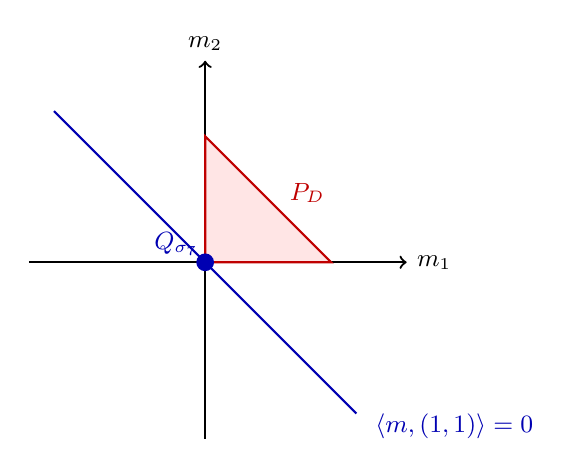
\begin{tikzpicture}[scale=1.6, line width=0.7pt, every node/.style={font=\small}]
          \draw[->, thick] (-1.4,0) -- (1.6,0) node[right] {$m_1$};
          \draw[->, thick] (0,-1.4) -- (0,1.6) node[above] {$m_2$};
          % Polytope P_D (the standard simplex)
          \fill[red!10] (0,0) -- (1,0) -- (0,1) -- cycle;
          \draw[red!75!black, thick] (0,0) -- (1,0) -- (0,1) -- cycle;
          \node[red!75!black, anchor=south west, inner sep=2pt] at (0.62,0.42) {$P_D$};
          % Line  <m, (1,1)> = 0  (i.e., m_1 + m_2 = 0)
          \draw[blue!70!black, thick] (-1.2,1.2) -- (1.2,-1.2);
          \node[blue!70!black, anchor=west, inner sep=2pt] at (1.30,-1.30) {$\langle m,(1,1)\rangle=0$};
          % Q_{sigma_7} = origin
          \fill[blue!70!black] (0,0) circle (2pt);
          \node[blue!70!black, anchor=south east, inner sep=2pt] at (0,0) {$Q_{\sigma_7}$};
        \end{tikzpicture}
        \caption{The face $Q_{\sigma_7}=\{m\in P_D:\langle m,(1,1)\rangle=0\}$ is the single point $\{(0,0)\}$, of dimension $0$ rather than the expected $1$.}
        \label{fig:Qsigma7}
    \end{figure}
    We find that $\dim Q_{\sigma_7}=0$, but the expected dimension is $2-1=1$. So the corresponding divisor, namely the exceptional divisor on $\Bl_0\mathbb{P}^2$ is in the non-Kähler locus. Similarly, we can verify that the non-Kähler locus consists only of this divisor.
\end{example}




Finally, we compute the mixed volumes of Newton bodies.
\begin{theorem}\label{thm:mix_vol_newbod}
Take $T$-invariant big divisors $D_1,\ldots,D_n$ on $X$. Consider $T_c$-invariant closed positive $(1,1)$-currents $T_i$ in $c_1(\mathcal{O}_X(D_i))$ for $i=1,\ldots,n$. Then
\begin{equation}\label{eq:mixvol_pob}
n! \vol \Bigl( \Delta(T_1),\ldots,\Delta(T_n) \Bigr)=\vol \left(T_1,\ldots,T_n \right).
\end{equation}
\end{theorem}
The mixed volume of currents is studied in \cref{sec:mix_vol}.
\begin{proof}
    It suffices to prove the following assertion:
    \begin{equation}\label{eq:Delta_add}
    \Delta(T_1+T_2)=\Delta(T_1)+\Delta(T_2).\footnotemark
    \end{equation}
    \footnotetext{This is slightly problematic when $n=1$, since $T_2$ is not defined \emph{stricto sensu}. We take $D_2,T_2$ satisfying the same assumptions as $D_1,T_1$ in this case.}
    In fact, assuming this, by induction, for each tuple of non-negative integers $C_1,\ldots,C_n$, we have
    \[
    \Delta\left( \sum_{i=1}^n C_i T_i \right)=\sum_{i=1}^n C_i \Delta(T_i).
    \]
    Comparing the volumes, we have
    \[
    \vol \Delta\left( \sum_{i=1}^n C_i T_i \right)=\sum_{i_1,\ldots,i_n=1}^n C_{i_1}\cdots C_{i_n} \vol \left(\Delta\left(T_{i_1}\right),\ldots,\Delta\left(T_{i_n}\right)\right).
    \]
    On the other hand, by \cref{prop:toricMAandrealMA2}, the $\mathcal{I}$-goodness of toric singularities \cref{ex:toricIgood}, and \cref{prop:vollinearlimit}, we have
    \[
    n! \vol \Delta\left( \sum_{i=1}^n C_i T_i \right)=\vol \left( \sum_{i=1}^n C_i T_i \right)=\sum_{i_1,\ldots,i_n=1}^n C_{i_1}\cdots C_{i_n} \vol \left(T_{i_1},\ldots,T_{i_n}\right).
    \]
    Comparing the coefficients of the above two expressions, we conclude \eqref{eq:mixvol_pob}.

    It only remains to establish \eqref{eq:Delta_add}. For this purpose, we fix smooth $T_c$-invariant Hermitian metrics $h_1$ and $h_2$ on $\mathcal{O}_X(D_1)$ and $\mathcal{O}_X(D_2)$ respectively. Correspondingly, take $h_1\otimes h_2$ as the reference Hermitian metric on $\mathcal{O}_X(D_1+D_2)$. Write
    \[
    \theta_1=\ddc h_1,\quad \theta_2=\ddc h_2.
    \]
    We choose the rational section of $\mathcal O_X(D_1+D_2)$ to be $s_{D_1}\otimes s_{D_2}$. With this choice and with the reference metric $h_1\otimes h_2$, the normalization \eqref{eq:normF0} gives
    \[
        F_{\theta_1+\theta_2}=F_{\theta_1}+F_{\theta_2}.
    \]
    Thus
    \[
        F_{\varphi_1+\varphi_2}=F_{\varphi_1}+F_{\varphi_2}.
    \]
    Take $\varphi_i\in \PSH_{\tor}(X,\theta_i)$ with $T_i=\theta_i+\ddc \varphi_i$ for $i=1,2$. Then $F_{\varphi_1}+F_{\varphi_2}$ is a candidate for $F_{\varphi_1+\varphi_2}$; see \eqref{eq:Fvarphibig1}. Therefore, \eqref{eq:Delta_add} follows from the equality of closed gradient images proved in \cref{lma:grad_img_sum}.
\end{proof}
